\chapter{二分类学习的可学习性}
\label{chap:binary-learnability}

一条规则把训练记录全部分对，为什么仍可能在新样本上出错？第~\ref{chap:statistical-learning-framework}章的垃圾邮件例子已经给出一个情形：阈值0.4和0.6都判对了四封训练邮件，却对分数落在0.4与0.6之间的邮件给出相反的判断，所以在这些邮件上二者至少有一个会出错。训练邮件恰好都没有落进这段区间，错误区域因而没有被观察到。样本的作用在于排除规则：一条规则只要在某封训练邮件上出错，就暴露了自己的错误区域；没有暴露，只说明错误区域还没被抽中。

一条错误率较高的规则，一般难以长期躲过检验；但学习算法是看过样本之后才在许多候选中挑选的。只要某一条坏规则碰巧通过了全部训练检验，算法就可能选中它。候选越多，至少一条坏规则侥幸通过的机会就越大。因此，本章首先控制有限候选中出现这种侥幸的概率，看它怎样随候选数和样本量变化（第~\ref{sec:binary-finite-class}节）。实数阈值有无穷多个，直接数候选就失去意义；但在有限个输入上，无穷多个阈值只能给出少数几种不同预测，算法在样本上能够区分的也只是这些预测。真正需要计数的，是有限输入上可区分的模式，打散、VC维与Sauer--Shelah引理刻画这些模式怎样随输入数增长（第~\ref{sec:binary-infinite-class}节）。

这条思路通向二分类可学习性的VC刻画（第~\ref{sec:binary-learnability-characterization}节）。VC维有限时模式只按多项式增长，借助一份不参与学习的副样本，就能同时控制全部候选的风险，这一侧解释怎样学会。VC维无限时，假设空间能在大量未见点上任意安排标签，训练样本给不出这些点的任何信息，任何学习器都会遇到信息不足，这一侧解释为什么有时学不会。最后，第~\ref{sec:computable-binary-learning}节区分三件事：统计上存在成功的学习器，程序能在有限步内找到输出，以及能否高效地找到输出。

全章沿用第~\ref{sec:learning-problem}节的二分类设定：每条观测$z=(x,y)$由输入$x\in X$和标签$y\in Y=\{0,1\}$组成，训练样本$S=(z_1,\ldots,z_n)\sim\mathcal P^n$独立同分布；预测错误计损失1，预测正确计损失0，即零一损失。于是总体风险与经验风险分别是
\[
 R_{\mathcal P}(h)=\mathbb P_{(x,y)\sim\mathcal P}\{h(x)\neq y\},\qquad
 \hat R_S(h)=\frac1n\sum_{i=1}^n\mathbb I\{h(x_i)\neq y_i\}.
\]
成功的标准是第~\ref{sec:pac-learning}节的可实现PAC（定义~\ref{def:realizable-pac}）与不可知PAC（定义~\ref{def:agnostic-pac}）。除非另行说明，比较决策空间与输出空间都取假设空间$\mathcal H$，即恰当学习；引用的外部结果若允许输出$\mathcal H$以外的分类器，会单独注明。

\section{有限假设空间}
\label{sec:binary-finite-class}

先考虑只含有限个假设的空间。仍以垃圾邮件过滤为例，假定学习算法只能在0.2、0.4、0.6、0.8这四个阈值中选择，分数不低于阈值的邮件判为垃圾邮件。邮件分数仍可以是$[0,1]$中的任意值，受限的只是可选的判定规则，于是假设空间只含四个假设。

把一条新观测看成对每个候选规则的一次检验：规则判对，就通过这次检验；判错，就在这封邮件上暴露一次错误。可实现时，存在一条总体上从不出错的正确规则，它不会因任何检验被排除；坏规则则只要被观察到一次错误就可以出局，所以只需担心坏规则一次也没被抓到。不可知时，每个候选都可能出错，见到一次错误就删除，可能把所有候选都删光，连最好的规则也留不下；这时要比较的是各候选的平均错误率，担心的是某个候选的训练错误比例明显低于它的总体风险。

两种分析使用同一个原则：先在抽样之前固定一个候选，计算它在样本上蒙混过关的概率；再对全部候选相加，以覆盖算法看过样本后作出的选择。两种情形要控制的失败事件不同，所需样本对精度的依赖也随之不同。

\subsection{可实现情形与一致学习}

本小节假定假设空间中存在一个总体风险为零的假设$h^\star$，即分布对$\mathcal H$可实现（定义~\ref{def:realizability}）。$h^\star$出错的概率为零，因此它几乎必然判对全部训练样本，ERM选出的假设训练错误也就为零。训练错误为零的假设称为与样本\term{一致}（consistent）。一致只说明这个假设判对了当前样本中的全部标签，不说明它在未见过的输入上也判对。

一致的假设仍可能有较高的总体风险。先看一个在抽样前固定、总体错误率为$0.1$的规则：一次检验未发现它出错的概率是$0.9$；各封邮件独立抽取，连续$n$次检验都未发现错误的概率是$0.9^n$。$n=10$时这个概率约为$0.35$，$n=44$时才降到1\%以下。一旦它通过了全部检验，它在训练样本上与$h^\star$同样没有错误，只看样本的ERM无法区分二者，可能选中它。

ERM面对的不止一条规则。把错误率至少为$0.1$的规则称为坏规则；我们事先不知道四个阈值中哪些是坏规则，只好把四个候选都算上；其中每个坏规则通过全部检验的概率都不超过$0.9^n$。ERM只要遇到其中任何一个蒙混过关就可能失败，所以要控制的是“至少一个坏规则仍然全对”这一事件。它是各个坏规则“全对”事件的并集，概率不超过各事件概率之和；坏规则不超过四个，所以这一概率至多为$4\times0.9^n$。这一步不要求各候选的检验结果相互独立：四个阈值在同一份样本上接受检验，结果显然相关，但并集的概率总不超过各部分概率之和。正因为并集界不管算法最终挑中了哪一个，它也覆盖了算法看过样本后才挑中的候选。图~\ref{fig:lt5-consistent-bad-survival}画出这些概率随$n$下降的情形：$4\times0.9^n$要到$n=57$才低于1\%，比单个规则多需要13个样本，这就是为“事后挑选”付出的代价。

\begin{figure}[htbp]
  \centering
  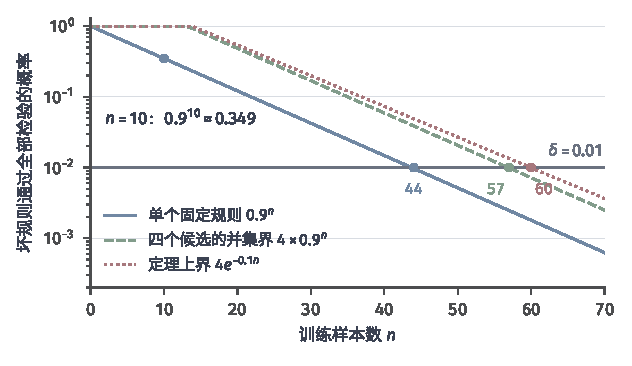
\includegraphics[width=107mm]{figures/06-foundations/02-learning-theory/matplotlib/lt5-consistent-bad-survival/figure.pdf}
  \caption{坏规则通过全部训练检验的概率。教学设定为四个候选阈值，坏规则指总体错误率至少为0.1的规则。蓝实线是一个错误率为0.1的固定规则判对$n$个独立样本的概率$0.9^n$；绿虚线是四个候选中至少一个坏规则判对全部样本的并集界$4\times0.9^n$；红点线是定理~\ref{thm:finite-realizable-pac}的上界$4e^{-0.1n}$，它用$1-\varepsilon\leq e^{-\varepsilon}$把乘积换成指数。纵轴为对数刻度，三条线分别在$n=44$、57、60时降到$\delta=0.01$以下。}
  \label{fig:lt5-consistent-bad-survival}
\end{figure}

下面把$0.1$换成任意给定的容限$\varepsilon$，把总体风险超过$\varepsilon$的假设称为高风险假设。先在抽样之前固定一个假设$h\in\mathcal H$。若$R_{\mathcal P}(h)>\varepsilon$，它判对一条随机观测的概率小于$1-\varepsilon$；各条观测独立，判对全部$n$条的概率等于各条概率之积：
\begin{equation}
  \mathbb P\bigl(\hat R_S(h)=0\bigr)
  =\bigl(1-R_{\mathcal P}(h)\bigr)^n
  \leq(1-\varepsilon)^n\leq e^{-n\varepsilon}.
  \label{eq:bad-consistent-hypothesis}
\end{equation}
最后一步用了$1-u\leq e^{-u}$，它把乘积换成便于反解的指数形式。式~\eqref{eq:bad-consistent-hypothesis}只适用于抽样之前固定的假设，ERM的输出依赖样本，不能直接代入。为此考察一个范围更大的事件：假设空间中至少有一个高风险假设与样本一致。如果ERM输出了高风险假设，这个输出本身与样本一致，上述事件必然发生；所以控制了这个事件的概率，就控制了ERM失败的概率。这个事件是各个高风险假设“与样本一致”事件的并集；并集界说它的概率不超过各事件概率之和，且不要求事件互斥，多个坏假设同时与样本一致并不影响结论。有限空间中至多有$|\mathcal H|$个高风险假设，由此得到下面的样本量界。

\begin{theorem}[有限假设空间的可实现PAC样本量界]
\label{thm:finite-realizable-pac}
设$(X,\mathcal X)$为可测空间，$Y=\{0,1\}$取离散$\sigma$代数，
$\mathcal H\subseteq Y^X$是由可测分类器组成的非空有限集合，$\mathcal P$是
$X\times Y$上的联合分布，采用零一损失下的$R_{\mathcal P}$与$\hat R_S$。
设$n\geq1$、$S=((x_i,y_i))_{i=1}^n\sim\mathcal P^n$，且存在
$h^\star\in\mathcal H$满足$R_{\mathcal P}(h^\star)=0$。对任意
$\varepsilon,\delta\in(0,1)$，若可测学习算法（允许内部随机性）以概率1输出满足
$\hat R_S(\hat h)=0$的$\hat h\in\mathcal H$，则
\begin{equation}
  \mathbb P_{S,A}\bigl(R_{\mathcal P}(\hat h)>\varepsilon\bigr)
  \leq |\mathcal H|e^{-n\varepsilon}.
  \label{eq:finite-realizable-failure}
\end{equation}
特别地，只要
\begin{equation}
  n\geq\frac{\log|\mathcal H|+\log(1/\delta)}{\varepsilon},
  \label{eq:finite-realizable-sample}
\end{equation}
算法就以至少$1-\delta$的概率输出期望风险不超过$\varepsilon$的假设；这里的概率
同时来自$S\sim\mathcal P^n$和算法的内部随机性。
\end{theorem}

\begin{proof}
题设保证输出几乎必然与样本一致；可实现性使$h^\star$几乎必然与样本一致，这样的选解因而存在。输出风险若超过$\varepsilon$，至少一个高风险假设与全部观测一致。由此
\begin{align*}
 \mathbb P\bigl(R_{\mathcal P}(\hat h)>\varepsilon\bigr)
 &\leq \mathbb P\bigl(\exists h\in\mathcal H:
       R_{\mathcal P}(h)>\varepsilon,\ \hat R_S(h)=0\bigr)\\
 &\leq\sum_{h:R_{\mathcal P}(h)>\varepsilon}
       \mathbb P\bigl(\hat R_S(h)=0\bigr)
 \leq |\mathcal H|e^{-n\varepsilon}.
\end{align*}
第一步是事件包含，第二步是并集界，第三步对每一项用式~\eqref{eq:bad-consistent-hypothesis}，并把高风险假设的个数放大为$|\mathcal H|$。令末项不超过$\delta$并取对数解出$n$，即得式~\eqref{eq:finite-realizable-sample}。
\end{proof}

定理的上界只用了候选总数和容限，没有用到哪些候选是坏规则、它们的错误率具体是多少，还把$(1-\varepsilon)^n$放大为$e^{-n\varepsilon}$，所以图~\ref{fig:lt5-consistent-bad-survival}中红点线位于另两条线之上：取$\varepsilon=0.1$、$\delta=0.01$，式~\eqref{eq:finite-realizable-sample}给出$\lceil(\log4+\log100)/0.1\rceil=60$，略多于并集界本身所需的57。再要求以至少99\%的概率得到总体风险不超过5\%的假设，即$\varepsilon=0.05$，充分样本量为$\lceil(\log4+\log100)/0.05\rceil=120$。这个样本量不依赖邮件分数和标签的具体分布：只要分布满足可实现条件，独立抽取120封邮件后，任何输出一致假设的算法都满足要求。

这里要分清三件事。一致只表示当前训练记录全部分对；定理保证的是，样本足够多时，全部分对的候选以高概率都是低风险的。样本量公式中，候选数以$\log|\mathcal H|$进入，容限以$1/\varepsilon$进入，置信度以$\log(1/\delta)$进入。所给的样本量是充分条件，不是精确的最小需求：定理没有说少于120封就一定达不到。

可选阈值增加到8个，容限和置信水平不变，充分样本量变为$\lceil(\log8+\log100)/0.05\rceil=134$。假设个数加倍，取整前的样本量只增加$\log2/\varepsilon\approx13.9$，因为候选数以对数形式进入。更一般地，对任意有限假设空间和任意$\varepsilon,\delta$，式~\eqref{eq:finite-realizable-sample}都给出一个不依赖分布的样本量，所以有限假设空间是可实现PAC可学习的。

这一论证依赖可实现性：零风险假设的存在保证ERM选得出一致假设，于是只需排除“高风险假设也与样本一致”这一种情况。若标签带有噪声，例如一部分邮件被人工误标，可能没有任何假设判对全部训练邮件，ERM比较的就不再是“有没有出错”，而是各假设出错比例的高低。总体风险较高的假设可能恰好在这份样本上错得较少而被选中。要排除这种情况，需要样本上的错误比例足够接近总体风险。

\subsection{不可知情形与一致收敛}
\label{sec:binary-uniform-convergence}

不可知情形下，假设空间中不一定存在零风险假设，学习的目标是使输出的总体风险接近$\mathcal H$中的最低水平$\inf_{h\in\mathcal H}R_{\mathcal P}(h)$。这时训练中出现错误，并不说明某个规则不值得选择：最好的阈值也可能错判几封误标的邮件。要判断的是它的平均错误率是否比其他候选更低，而训练错误比例只是总体错误率的一个估计。于是问题变成：这些估计有多可信。

先看一个在抽样前固定的假设$h$。每条观测上的零一损失取值0或1，均值为$R_{\mathcal P}(h)$；$n$条观测的损失相互独立，所以经验风险是$n$个独立Bernoulli随机变量的平均。Hoeffding不等式说，独立且取值有界的随机变量，其平均值偏离均值的概率随样本量指数下降，速度只取决于取值区间的长度（定理与证明可参考\BookChapterRef{chap:random-sequences-and-processes}{卷3《数学准备：优化、动力系统与信号处理》的“随机序列与随机过程”章}）。对取值于$[0,1]$的损失，它给出
\begin{equation}
 \mathbb P\left(\left|\hat R_S(h)-R_{\mathcal P}(h)\right|>\eta\right)
 \leq2e^{-2n\eta^2}.
 \label{eq:hoeffding-fixed-hypothesis}
\end{equation}
例如$n=1000$、$\eta=0.05$时，右侧为$2e^{-5}\approx0.013$。

式~\eqref{eq:hoeffding-fixed-hypothesis}同样只适用于抽样前固定的假设，不能直接用于依赖样本的输出$A(S)$。以四个阈值为例，ERM计算四个经验风险并选出最小者。每个估计各自以高概率准确，并不排除这一次恰有某个估计偏低；而ERM正是偏向挑中估计偏低的候选，因为偏低的估计让它看起来更好。图~\ref{fig:learning-uniform-convergence}中，每条竖线表示一个假设的经验风险与总体风险之差；ERM恰好选中了竖线最长、经验风险被低估最多的那一个。只有全部竖线同时都短，ERM看过数据后选中的那个估计才一定可信。从“每个估计各自可信”到“看过数据后选中的估计也可信”，需要对全部候选同时控制偏差。

\begin{figure}[htbp]
  \centering
  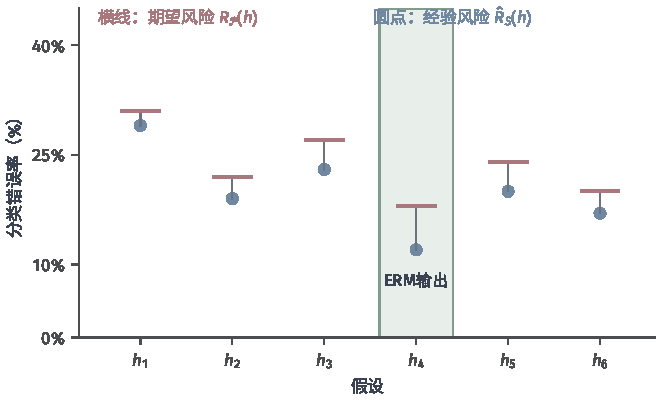
\includegraphics[width=107mm]{figures/06-foundations/02-learning-theory/matplotlib/learning-theory-uniform-convergence/figure.pdf}
  \caption{单个风险估计与共同保证。竖线连接各假设的经验风险与期望风险；只限制其中一条线，不能覆盖ERM在框中选择的输出。限制全部竖线后，这个数据依赖输出也落在保证内。}
  \label{fig:learning-uniform-convergence}
\end{figure}

因此需要这样一种保证：同一份样本以高概率同时把所有假设的风险估计准确，所需样本量对所有联合分布统一适用。

\begin{definition}[一致收敛]
\label{def:learning-uniform-convergence}
称二分类假设空间$\mathcal H$在零一损失下满足\term{一致收敛}（uniform convergence），是指对任意$\eta,\delta\in(0,1)$，存在只依赖$\mathcal H,\eta,\delta$的样本量$m_{\mathcal H}^{\mathrm{UC}}(\eta,\delta)$，使得对$X\times Y$上的任意联合分布$\mathcal P$和任意$n\geq m_{\mathcal H}^{\mathrm{UC}}(\eta,\delta)$，都有
\begin{equation}
 \mathbb P_{S\sim\mathcal P^n}\left(
   \sup_{h\in\mathcal H}|\hat R_S(h)-R_{\mathcal P}(h)|\leq\eta
 \right)\geq1-\delta.
 \label{eq:learning-uniform-convergence-definition}
\end{equation}
\end{definition}

上确界不超过$\eta$，意味着每个假设在这份样本上的偏差都不超过$\eta$，上确界本身不必由某个假设取到。概率保证允许偶尔抽到偏差较大的样本，只要这种样本出现的概率不超过$\delta$。不同分布下各假设的总体风险不同，样本量却必须对所有分布同时适用；定义不要求存在零风险假设，所以它覆盖不可知设定。一致收敛要求的是风险估计准确，并不要求风险小：一个总体风险为40\%的假设，只要样本上的错误比例也接近40\%，就满足要求；从中挑出风险小的假设，是ERM的事。

对有限空间，只要每个候选的损失函数可测，上确界就是有限个可测随机变量的最大值，因而可测，式~\eqref{eq:learning-uniform-convergence-definition}中的概率及相应的偏差事件都有定义。第~\ref{sec:measurability-convention}节为无限假设空间准备的可测性约定，在有限情形用不到。“所有偏差都不超过$\eta$”的反面是“至少一个假设的偏差超过$\eta$”，对有限个假设应用并集界，就得到下面的定理。

\begin{theorem}[有限假设空间的一致收敛样本量界]
\label{thm:finite-uniform-convergence}
设$(X,\mathcal X)$为可测空间，$Y=\{0,1\}$取离散$\sigma$代数，
$\mathcal H\subseteq Y^X$是由可测分类器组成的非空有限集合，$\mathcal P$是
$X\times Y$上的任意联合分布，采用零一损失。
设$n\geq1$且$S=((x_i,y_i))_{i=1}^n\sim\mathcal P^n$。对任意
$\eta,\delta\in(0,1)$，只要样本量满足
\begin{equation}
 n\geq\frac{\log(2|\mathcal H|/\delta)}{2\eta^2},
 \label{eq:finite-uniform-sample}
\end{equation}
就有
\[
 \mathbb P_{S\sim\mathcal P^n}\left(
 \sup_{h\in\mathcal H}|\hat R_S(h)-R_{\mathcal P}(h)|\leq\eta
 \right)\geq1-\delta.
\]
同一概率界也可写为：对任意$n\geq1$和$\delta\in(0,1)$，以下不等式以至少$1-\delta$的概率成立：
\begin{equation}
 \sup_{h\in\mathcal H}|\hat R_S(h)-R_{\mathcal P}(h)|
 \leq\sqrt{\frac{\log(2|\mathcal H|/\delta)}{2n}}.
 \label{eq:finite-uniform-bound}
\end{equation}
由于该样本量不依赖$\mathcal P$，有限假设空间满足一致收敛。
\end{theorem}

\begin{proof}
对每个$h$使用式~\eqref{eq:hoeffding-fixed-hypothesis}。上确界超过$\eta$等价于至少一个假设的偏差超过$\eta$；对这些事件求并集界，得到
\[
 \mathbb P\left(\sup_{h\in\mathcal H}|\hat R_S(h)-R_{\mathcal P}(h)|>\eta\right)
 \leq 2|\mathcal H|e^{-2n\eta^2}.
\]
按式~\eqref{eq:finite-uniform-sample}选择$n$使右侧至多为$\delta$；或令右侧等于$\delta$反解$\eta$，得到式~\eqref{eq:finite-uniform-bound}。两种写法的样本要求均与具体$\mathcal P$无关。
\end{proof}

一致收敛给出了“所有假设同时估计准确”的事件，接下来要把它转成ERM的风险保证。第~\ref{sec:risk-comparison}节已经对一般损失建立了这一步（定理~\ref{thm:approximate-erm-risk}）：若同一份样本上所有候选的总体—经验偏差都不超过$\eta$，而算法输出的经验风险至多比类内经验下确界高$\alpha$，则输出的总体风险至多比类内最低总体风险高$2\eta+\alpha$。精确ERM对应$\alpha=0$。对四个阈值，这三步比较是：从输出的总体风险换到它的经验风险，误差至多$\eta$；输出的经验风险不高于任一参照阈值的经验风险；再从参照的经验风险换回它的总体风险，误差又至多$\eta$。取$\eta=\varepsilon/2$，便得到下面的不可知样本量。

\begin{theorem}[有限假设空间的不可知PAC样本量界]
\label{thm:finite-agnostic-pac}
设$(X,\mathcal X)$为可测空间，$Y=\{0,1\}$取离散$\sigma$代数，
$\mathcal H\subseteq Y^X$是由可测分类器组成的非空有限集合，$\mathcal P$是
$X\times Y$上的任意联合分布，采用零一损失。
设$n\geq1$、$S=((x_i,y_i))_{i=1}^n\sim\mathcal P^n$，可测学习算法
$A$（允许内部随机性）以概率1输出
$\hat h=A(S)\in\argmin_{h\in\mathcal H}\hat R_S(h)$。对任意
$\varepsilon,\delta\in(0,1)$，只要
\begin{equation}
 n\geq\frac{2}{\varepsilon^2}
 \left(\log(2|\mathcal H|)+\log\frac1\delta\right),
 \label{eq:finite-agnostic-sample}
\end{equation}
就有
\[
 \mathbb P_{S,A}\left(
 R_{\mathcal P}(\hat h)\leq\inf_{h\in\mathcal H}R_{\mathcal P}(h)+\varepsilon
 \right)\geq1-\delta.
\]
概率同时来自样本抽取和$A$的内部随机性。
\end{theorem}

\begin{proof}
在定理~\ref{thm:finite-uniform-convergence}中取$\eta=\varepsilon/2$。式~\eqref{eq:finite-agnostic-sample}正是式~\eqref{eq:finite-uniform-sample}在这一容限下的形式，所以全部偏差不超过$\varepsilon/2$的事件概率至少为$1-\delta$。在这个事件上，输出$\hat h$也在$\mathcal H$内，同样受偏差界约束；ERM给出$\alpha=0$。由定理~\ref{thm:approximate-erm-risk}，$R_{\mathcal P}(\hat h)\leq\inf_{h\in\mathcal H}R_{\mathcal P}(h)+2\cdot\varepsilon/2$。有限空间中经验风险的最小值总能取到，所以ERM输出存在。
\end{proof}

这个定理控制的是超额风险，即输出比$\mathcal H$中最低总体风险高出多少；它没有说最低风险本身小。若阈值空间的最低风险是12\%，定理只保证输出不超过$12\%+\varepsilon$。

\subsection{两种样本量界的比较}

两个定理的样本量中，精度分别以$1/\varepsilon$和$1/\varepsilon^2$进入。这一差别来自两种情形要控制的失败事件不同。可实现时，要排除的是这样的规则：它的错误区域概率质量超过$\varepsilon$，却始终没被$n$次抽样命中。每次抽样命中错误区域的概率至少为$\varepsilon$，平均每$1/\varepsilon$个样本就会命中一次，所以$n$达到$1/\varepsilon$的若干倍时，这样的规则几乎一定露出马脚，漏网的概率按$e^{-n\varepsilon}$下降，精度只以一次幂进入样本量。不可知时，各候选通常都会出错，要做的是把每个错误率估计的波动压到$\varepsilon$量级。样本错误比例的标准差约为$1/\sqrt n$量级，要使它小于$\varepsilon/2$，就需要$n$与$1/\varepsilon^2$同阶，对应式~\eqref{eq:hoeffding-fixed-hypothesis}中指数里的$n\eta^2$，精度以二次幂进入样本量。

保持同一候选集合和置信度，用数字看这一差别。$|\mathcal H|=4$、$\delta=0.01$时，$\varepsilon=0.1$的可实现充分样本量是60，不可知是1337；$\varepsilon=0.05$时分别是120和5348。图~\ref{fig:lt5-finite-sample-size-comparison}显示，$\varepsilon$每减半，前者翻一倍，后者变为四倍：两条线在对数坐标下的斜率分别为1和2。

\begin{figure}[htbp]
  \centering
  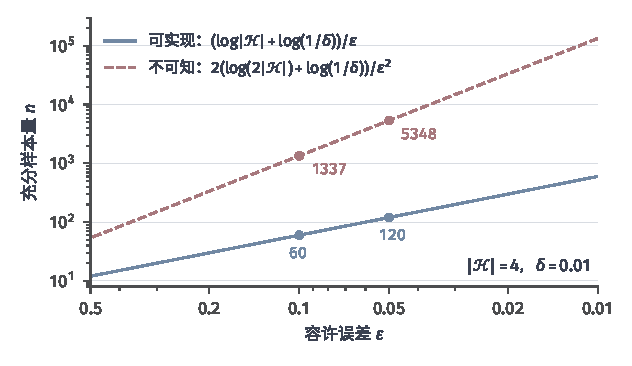
\includegraphics[width=107mm]{figures/06-foundations/02-learning-theory/matplotlib/lt5-finite-sample-size-comparison/figure.pdf}
  \caption{有限类两种充分样本量随容许误差的变化。$|\mathcal H|=4$，$\delta=0.01$；蓝实线为定理~\ref{thm:finite-realizable-pac}的可实现样本量，红虚线为定理~\ref{thm:finite-agnostic-pac}的不可知样本量。横轴从左到右误差变小，两轴均为对数刻度；标注点为$\varepsilon=0.1$与$0.05$时取整后的数值。}
  \label{fig:lt5-finite-sample-size-comparison}
\end{figure}

这一比较针对的是本章所用的两个一般保证，并不断言任意含噪问题都需要$1/\varepsilon^2$量级的样本。例如，若最好的候选错误率很低，估计在它附近的波动也小，专门的分析可以得到介于两者之间的样本量\scite{shalevshwartz2014}；这类细化本章不展开。至于在最坏分布下是否任何算法都摆脱不了二次幂，需要信息下界来回答，第~\ref{sec:binary-learnability-characterization}节的定理~\ref{thm:binary-optimal-sample-complexity}引用了相应的最优阶。

两种界中，候选数都以$\log|\mathcal H|$进入：这是为“看过样本再选”付出的统计代价。候选数加倍，可实现样本量只增加$\log2/\varepsilon$，在$\varepsilon=0.05$时约为14个；不可知样本量增加$2\log2/\varepsilon^2$，约为555个。这一代价与算法搜索候选的计算成本是两回事：逐个计算经验风险需要$n|\mathcal H|$次损失评估，候选数加倍时这一计算量也加倍，而不是只增加一个对数项。有限计数回答了统计问题，却留下两件事：实数阈值有无穷多个，$\log|\mathcal H|=\infty$使上面的界失去意义；候选数随问题规模指数增长时，逐个搜索也不可行。前者是下一节的问题，后者留到第~\ref{sec:computable-binary-learning}节。若候选来自多个空间、需要为每个空间分配失败概率，相应的分配与编码方法见第~\ref{sec:srm}节。

\section{无限假设空间的组合结构}
\label{sec:binary-infinite-class}
\label{sec:comb-label-family-capacity}

有限空间的样本量界中，$\log|\mathcal H|$来自并集界对每个候选各付一次失败概率。全体实数阈值有无穷多个，这一项变成无穷，界什么也说明不了。但失效来自计数方式，不一定来自问题本身。四个有序输入把实数轴分成五段，阈值只能落在其中一段；在同一段内移动阈值，这四点上的预测一个也不变。阈值0.500与0.501便是如此：它们只在分数落在二者之间的邮件上预测不同，并集界却把两者的失败概率当作互不重叠的部分重复相加。所以直接数参数或规则总数可能过于粗糙，本节改为数有限输入上真正不同的预测模式。

本节的定义按这一需要依次给出。限制类与生长函数把“真正不同的预测模式”写成能够逐个数出的对象；打散检查某组输入上的模式能否完全自由组合，VC维记录这种自由组合最多能覆盖几个点；Sauer--Shelah引理再把这一局部的自由度变成模式数的统一上界。这些组合量怎样进入关于总体风险的概率界，是第~\ref{sec:binary-learnability-characterization}节的任务。

\subsection{限制类与生长函数}
\label{sec:comb-binary-restrictions}

训练邮件的分数为0.1、0.3、0.7、0.9时，凡是大于0.3且不超过0.7的阈值，都把前两封判为正常邮件、后两封判为垃圾邮件；它们在这四封邮件上的预测完全相同，经验风险也相同。对右侧判正的阈值，按阈值所在的区间逐段列出四点上的预测：阈值超过0.9时得到$0000$，落在$(0.7,0.9]$时得到$0001$，落在$(0.3,0.7]$时得到$0011$，落在$(0.1,0.3]$时得到$0111$，不超过0.1时得到$1111$。这里把四点上的预测按分数从小到大写成一个串，例如$0011$即预测向量$(0,0,1,1)$。无穷多个阈值就这样被四个观测分成五组，图~\ref{fig:lt5-threshold-four-point-patterns}逐行画出。全部可能的二元组合有$2^4=16$种，其余11种，例如$1011$，任何阈值都给不出：一封邮件被判为垃圾，分数更高的邮件也必被判为垃圾。

\begin{figure}[htbp]
  \centering
  % 无穷多个阈值在四个训练分数上只给出五种预测模式（第5章5.2.1）。
% 训练分数 0.1、0.3、0.7、0.9；阈值规则 h_t(x)=I{x>=t}，t in [0,1]。
% 小数轴映射：屏幕横坐标 = 34 + 50*s（s 为分数），每行用色带标出给出该模式的阈值段。
% 实心蓝点为预测 1，空心红圈为预测 0；第三行另标 t=0.5 与 t=0.6 两个具体阈值。
\begingroup
\providecolor{FigureGreen}{HTML}{829C8B}
\providecolor{FigureGreenFill}{HTML}{E8EEE9}
\begin{tikzpicture}[figure picture,x=1mm,y=1mm,
  one/.style={circle,fill=FigureBlue,draw=FigureBlue,inner sep=0pt,minimum size=2.6mm},
  zero/.style={circle,fill=white,draw=FigureRed,line width=.75pt,inner sep=0pt,minimum size=2.6mm}]
\node[figure heading,anchor=west] at (0,49) {阈值所在区间};
\node[figure heading] at (59,49) {四封邮件上的预测};
\node[figure heading] at (98,49) {模式};
\foreach \x/\s in {39/0.1,49/0.3,69/0.7,79/0.9}{\node[figure note] at (\x,44) {$\s$};}
\foreach \row/\lab/\a/\b/\pa/\pb/\pc/\pd/\pat in {
  0/{$t\leq0.1$}/34/39/one/one/one/one/{(1,1,1,1)},
  1/{$0.1<t\leq0.3$}/39/49/zero/one/one/one/{(0,1,1,1)},
  2/{$0.3<t\leq0.7$}/49/69/zero/zero/one/one/{(0,0,1,1)},
  3/{$0.7<t\leq0.9$}/69/79/zero/zero/zero/one/{(0,0,0,1)},
  4/{$0.9<t\leq1$}/79/84/zero/zero/zero/zero/{(0,0,0,0)}}{
  \pgfmathsetmacro{\y}{38-9*\row}
  \node[anchor=west] at (0,\y) {\lab};
  \fill[FigureGreenFill] (\a,\y-2.2) rectangle (\b,\y+2.2);
  \draw[FigureGreen,line width=.9pt] (\a,\y+2.2)--(\b,\y+2.2);
  \draw[FigureStroke] (34,\y)--(84,\y);
  \node[\pa] at (39,\y) {};\node[\pb] at (49,\y) {};
  \node[\pc] at (69,\y) {};\node[\pd] at (79,\y) {};
  \node at (98,\y) {\pat};
}
\foreach \x/\t in {59/{0.5},64/{0.6}}{
  \draw[FigureInk,line width=.75pt] (\x,18.6)--(\x,21.4);
  \node[figure note] at (\x,16) {$\t$};}
\end{tikzpicture}
\endgroup

  \caption{无穷多个阈值在四个输入上的五种预测模式。每行的绿色色带是给出该行模式的全部阈值所在的区间，实心蓝点表示预测1（垃圾邮件），空心红圈表示预测0。第三行中阈值0.5与0.6落在同一色带内，在这四封邮件上不可区分。}
  \label{fig:lt5-threshold-four-point-patterns}
\end{figure}

这种归类可以对任意假设空间和任意有限输入进行。固定有限个输入，只保留每个假设在这些位置上的输出，即使假设空间无限大，当前能区分的输出记录也只有有限种。

\begin{definition}[限制类]
\label{def:restriction-class}
设$C=\{x_1,\ldots,x_m\}$为互异输入组成的有限集，并固定所列次序。把每个假设在这些输入上的取值组成一个向量，所有这样的向量构成$\mathcal H$在$C$上的\term{限制}（restriction）类：
\[
 \mathcal H|_C=\{(h(x_1),\ldots,h(x_m)):h\in\mathcal H\}.
\]
\end{definition}

限制类中的一个向量称为一个可实现的预测模式。不同假设若在$C$上取值相同，只在限制类中计一次；限制类是$\{0,1\}^m$的子集，至多有$2^m$个模式，无论$\mathcal H$本身有多大。阈值0.5与0.6都给出$(0,0,1,1)$，却在两个训练分数之间的0.55上取值不同：当前模式相同，不等于两个假设相同。正因如此，限制类本身只是有限输入上的计数；总体风险由整个分布决定，两个在样本上不可区分的假设，总体风险可以不同。

限制类的大小依赖$C$的位置，而我们事先不知道样本会落在哪里。为得到对所有分布都适用的保证，对$m$个输入的所有选法取最坏情形。

\begin{definition}[生长函数]
\label{def:growth-function}
\term{生长函数}（growth function）记录$m$个输入上最多能区分多少种模式。对整数$m\geq0$，定义
\begin{equation}
 \Pi_{\mathcal H}(m)
 =\max_{x_1,\ldots,x_m\in X}
   \left|\{(h(x_1),\ldots,h(x_m)):h\in\mathcal H\}\right|.
 \label{eq:growth-function}
\end{equation}
$m=0$时只有一个空模式，故$\Pi_{\mathcal H}(0)=1$。
\end{definition}

定义允许输入重复，因此即使输入空间有限，生长函数对任意$m$也有定义；重复的位置必须取相同的标签，模式只会更少，所以最大值总可以在互异输入上取到（当$X$至少有$m$个点时）。模式数是$1$到$2^m$之间的整数，有限个整数中总有最大者，所以定义中的最大值存在。有限空间总有$\Pi_{\mathcal H}(m)\leq|\mathcal H|$，生长函数因此是假设个数的推广：它只计入在这$m$个输入上能够区分的假设。

阈值空间的生长函数可以直接数出来。把$m$个互异分数从小到大排为$x_1<\cdots<x_m$，模式只取决于阈值落在$(-\infty,x_1]$、$(x_1,x_2]$、$\ldots$、$(x_m,\infty)$中的哪一段，共$m+1$段，每段给出不同的模式，所以$\Pi_{\mathcal H}(m)=m+1$。图~\ref{fig:lt5-threshold-four-point-patterns}是$m=4$的情形。

到这里得到的只是有限输入上的计数：生长函数说明$m$个输入上至多出现多少种预测，却没有说明这些预测在未见输入上的表现，因而还不能直接代入涉及总体风险的概率事件。第~\ref{sec:binary-learnability-characterization}节会用一份副样本补上这一步。

\subsection{打散与VC维}
\label{sec:binary-shattering-vc}
\label{sec:comb-vc-growth}
\label{sec:comb-binary-shattering-counts}

学习要靠已见标签约束未见标签。于是可以问：在一组输入上，知道其中一部分点的标签，能否约束同一组中其余点的标签？对阈值能：四个分数0.1、0.3、0.7、0.9中，若已知0.3被判为1，则0.7和0.9也必被判为1，五种模式里只剩两种与之相容。另一种极端是，这组输入上全部$2^m$种二元标记都可实现，限制类达到平凡上界$2^m$个模式。这时固定已见点的任何标签，其余每个点仍能任意二选一，因为每种延续方式都有假设实现；已见标签对同组的其余点不提供任何约束。注意这种歧义只限定在这组输入之内，并不说明假设空间在任意外部输入上也同样自由。第~\ref{sec:no-free-lunch}节没有免费的午餐定理利用的正是这种情形。

\begin{definition}[打散]
\label{def:shattering}
若对有限互异输入集$C=\{x_1,\ldots,x_m\}$的每个二值标记$(b_1,\ldots,b_m)$，都存在$h\in\mathcal H$满足$h(x_i)=b_i$对全部$i$成立，就称$\mathcal H$\term{打散}（shatter）$C$。等价地，$\mathcal H|_C=\{0,1\}^m$。
\end{definition}

若每个$m$都有能被打散的$m$点集合，$\log\Pi_{\mathcal H}(m)=m\log2$随$m$线性增长；第~\ref{sec:binary-learnability-characterization}节会看到，它在概率界中起着$\log|\mathcal H|$的作用，线性增长会抵消样本增多带来的集中效果。所以要关心的是：能被打散的点集最多有多大。

\begin{definition}[VC维]
\label{def:vc-dimension}
$\mathcal H$的\term{VC维}（Vapnik--Chervonenkis dimension）为
\[
 \operatorname{VC}(\mathcal H)
 =\sup\{|C|:C\subseteq X,\ |C|<\infty,\ C\text{被}\mathcal H\text{打散}\}.
\]
空集总能被非空假设空间打散，所以VC维可为$0$；若任意大的有限集都能被打散，则取值为$+\infty$。
\end{definition}

等价地，$\operatorname{VC}(\mathcal H)$是满足$\Pi_{\mathcal H}(m)=2^m$的最大$m$。白话地说，VC维是假设空间能够任意贴合标签的最大点数。这一量词结构决定了两个方向的证明各需要什么：证明$\operatorname{VC}(\mathcal H)\geq d$只需找到一组$d$个完全自由的点，即一个被打散的$d$点集合；证明$\operatorname{VC}(\mathcal H)\leq d$则要说明再多一个点时总有某种标记无法实现，即对每组$d+1$个点都指出一种实现不了的标记。前者是“存在”，后者是“任意”，难度通常不对称。

VC维不是参数个数。$h_{a,b}(x)=\mathbb I\{x\geq a+b\}$写成两个参数，实现的仍是同一个阈值空间，VC维仍为1：不同的参数表示可以对应同一个预测类，而VC维只看预测类。反过来，一个参数也可以产生无穷的VC维。取$X=\mathbb N$，对每个自然数$k$令$h_k(x)$为$k$的二进制展开中第$x$位上的数字（从第0位数起）。任给有限集$C\subseteq\mathbb N$及其标记$b$，取$k=\sum_{x\in C,\ b_x=1}2^x$，则$h_k$在$C$上恰好实现$b$；所以这个只由一个整数索引的类打散任意有限集，VC维为无穷。参数个数衡量的是描述方式，VC维衡量的是预测类在有限输入上的组合自由度。VC维此时只是类的一个结构量；它是否刻画可学习性，要等第~\ref{sec:binary-learnability-characterization}节的概率论证。

\subsection{阈值、区间与半空间的例子}

下面三个例子都按上述两个方向检查：先构造一组完全自由的点，再具体找出多一个点时缺失的标记。缺失的标记正是几何约束限制标签独立选择的地方。

\paragraph{阈值与区间}
递增阈值空间取整个实数输入空间并允许所有实数阈值，分数不低于阈值时预测1。把阈值放在单个点的左侧或右侧，就能实现该点的两种标签，所以单点集被打散，VC维至少为1。对任意两个分数$x_1<x_2$，“左正右负”的标记$10$实现不了，因为$x_1$达到阈值时$x_2$也达到；所以没有两点集被打散，VC维为1。前一小节已算出$\Pi_{\mathcal H}(m)=m+1$。

单个区间（区间内预测1）能打散两个点：$x_1<x_2$上的四种标记分别由空区间、只含$x_2$的区间、只含$x_1$的区间和同时包含二者的区间实现。三个点$x_1<x_2<x_3$上的$101$实现不了，因为包含$x_1$和$x_3$的区间必然包含$x_2$，所以VC维为2。区间在$m$个不同点上的预测由它覆盖哪一段连续的点决定：覆盖为空有1种，非空时由首尾两点确定，有$m(m+1)/2$种，合计
\[
 \Pi_{\mathcal H}(m)=1+\frac{m(m+1)}2.
\]
$m=3$时为7，正好比$2^3=8$少了$101$这一种。图~\ref{fig:comb-interval-shattering-patterns}并列显示阈值与区间的这两项判断。

\begin{figure}[htbp]
  \centering
  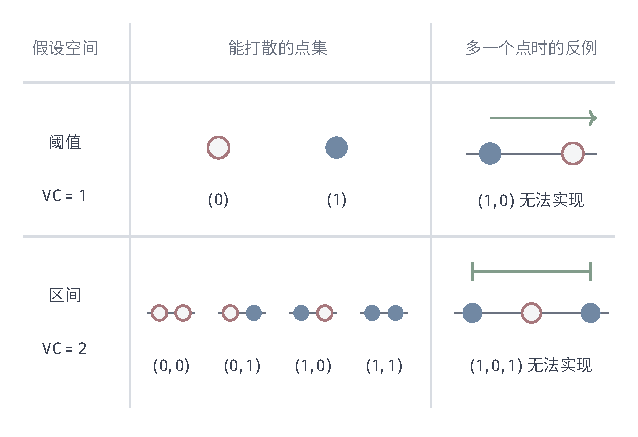
\includegraphics[width=107.999mm]{figures/06-foundations/02-learning-theory/tikz/comb-interval-shattering-patterns/figure.pdf}
  \caption{阈值与单区间函数类的VC维。中列给出能够打散的输入和相应模式；
 右列给出多一个输入时无法实现的模式。实心点表示标签$1$，空心点表示标签$0$；
 箭头表示阈值的正标签向右延续，线段表示包含两个端点的区间也包含中间点。}
 \label{fig:comb-interval-shattering-patterns}
 \label{fig:learning-vc-shattering}
 \label{fig:learning-vc-dimension-examples}
\end{figure}

\paragraph{平面上的半空间}
平面上的仿射半空间分类器为$h_{\bm w,b}(\bm x)=\mathbb I\{\langle\bm w,\bm x\rangle+b\geq0\}$，其中$\bm w\in\mathbb R^2$、$b\in\mathbb R$；它把一条直线一侧（含直线）判为1。它的VC维为3。

下界方向，取三个不共线的点。图~\ref{fig:lt5-halfplane-shattering}左侧逐格画出全部8种标记及实现它们的一条分界线：单点为1时，用一条直线把该点与另两点分开；两点为1时，把第三点单独隔开并取另一侧；全0和全1分别取不含、包含三点的半平面。三点不共线，保证任意一点都能被一条直线单独隔开。

上界方向，要说明任意四个点都有一种标记实现不了。任取四个点，只有两种情形：要么其中一点落在其余三点的凸包内（三点共线时中间那一点就落在另两点连成的线段上，也属于这种情形），要么四点构成凸四边形。前一种情形下，把外围三点标为1、内部点标为0实现不了：半平面是凸集，包含三点就包含它们的凸包。后一种情形下，两条对角线相交于一点；把一条对角线的两端标为1、另一条的两端标为0，则预测1的半平面包含第一条对角线及其上的交点，预测0的一侧是开半平面，同样是凸集，包含第二条对角线及同一个交点，同一个点不能同时属于两侧，矛盾。图~\ref{fig:lt5-halfplane-shattering}右侧画出这两种情形。

\begin{figure*}[htbp]
  \centering
  % 平面仿射半空间 h_{w,b}(x)=I{<w,x>+b>=0} 的打散与不可实现标记（第5章5.2.3）。
% 左侧：不共线三点 P1=(5,3)、P2=(15,3)、P3=(9,12)（各 20x16 小格的局部坐标，单位 mm）上的全部 8 种标记，
%   每格画出一条实现该标记的分界线，浅蓝区域为预测 1 的半平面；全 0 与全 1 用整体偏移的半平面实现。
%   分界线：{P1}: 过 (9,0) 与 (0,9)；{P2}: 过 (11,0) 与 (20,9)；{P3}: y=8；{P1,P2}: y=7；{P1,P3}: 过 (12,0) 与 (16,16) 的直线左侧；{P2,P3}: 过 (10,0) 与 (3,16) 的直线右侧。
% 右侧：四点的两种几何情形。(a) D=(10,6) 在 A=(0,0)、B=(20,0)、C=(10,16) 的凸包内，标记 A,B,C 为 1、D 为 0 不可实现；
%   (b) 凸四边形 E=(0,0)、F=(20,4)、G=(16,16)、K=(2,12)，对角线 EG（y=x）与 FK 交于 (116/13,116/13)≈(8.92,8.92)，
%   标记 E,G 为 1、F,K 为 0 不可实现。实心蓝点为 1，空心红圈为 0。
\begingroup
\begin{tikzpicture}[figure picture,x=1mm,y=1mm,
  one/.style={circle,fill=FigureBlue,draw=FigureBlue,inner sep=0pt,minimum size=2.3mm},
  zero/.style={circle,fill=white,draw=FigureRed,line width=.75pt,inner sep=0pt,minimum size=2.3mm},
  cut/.style={draw=FigureStroke,line width=.75pt},
  hp positive/.style={fill=FigureBlueFill}]
\node[figure heading,anchor=west] at (0,47) {不共线的三点：8 种标记都可实现};
% 小格辅助命令：#1,#2 为小格原点，#3 填色，#4 分界线，#5 三个点，#6 小格说明。
\newcommand{\hpPanel}[6]{% #1 ox, #2 oy, #3 fill path (relative), #4 cut path, #5 labels P1..P3 styles as a/b/c, #6 caption
  \begin{scope}[shift={(#1,#2)}]
    \begin{scope}\clip (0,0) rectangle (20,16); #3 \end{scope}
    \draw[FigureGrid,line width=.5pt] (0,0) rectangle (20,16);
    #4
    #5
    \node[figure note] at (10,-3.2) {#6};
  \end{scope}}
% points in panel coords: P1=(5,3) P2=(15,3) P3=(9,12)
\def\Pa{(5,3)}\def\Pb{(15,3)}\def\Pc{(9,12)}
\hpPanel{0}{24}{}{}{\node[zero] at \Pa{};\node[zero] at \Pb{};\node[zero] at \Pc{};}{全为 0}
\hpPanel{24}{24}{\fill[hp positive] (0,0)--(9,0)--(0,9)--cycle;}{\draw[cut] (9,0)--(0,9);}{\node[one] at \Pa{};\node[zero] at \Pb{};\node[zero] at \Pc{};}{$P_1$ 为 1}
\hpPanel{48}{24}{\fill[hp positive] (11,0)--(20,0)--(20,9)--cycle;}{\draw[cut] (11,0)--(20,9);}{\node[zero] at \Pa{};\node[one] at \Pb{};\node[zero] at \Pc{};}{$P_2$ 为 1}
\hpPanel{72}{24}{\fill[hp positive] (0,8)rectangle(20,16);}{\draw[cut] (0,8)--(20,8);}{\node[zero] at \Pa{};\node[zero] at \Pb{};\node[one] at \Pc{};}{$P_3$ 为 1}
\hpPanel{0}{0}{\fill[hp positive] (0,0)rectangle(20,7);}{\draw[cut] (0,7)--(20,7);}{\node[one] at \Pa{};\node[one] at \Pb{};\node[zero] at \Pc{};}{$P_1,P_2$ 为 1}
\hpPanel{24}{0}{\fill[hp positive] (0,0)--(12,0)--(16,16)--(0,16)--cycle;}{\draw[cut] (12,0)--(16,16);}{\node[one] at \Pa{};\node[zero] at \Pb{};\node[one] at \Pc{};}{$P_1,P_3$ 为 1}
\hpPanel{48}{0}{\fill[hp positive] (10,0)--(20,0)--(20,16)--(3,16)--cycle;}{\draw[cut] (10,0)--(3,16);}{\node[zero] at \Pa{};\node[one] at \Pb{};\node[one] at \Pc{};}{$P_2,P_3$ 为 1}
\hpPanel{72}{0}{\fill[hp positive] (0,0)rectangle(20,16);}{}{\node[one] at \Pa{};\node[one] at \Pb{};\node[one] at \Pc{};}{全为 1}
\node[figure note,anchor=west] at (0,42.5) {$P_1$ 左下，$P_2$ 右下，$P_3$ 居上；浅蓝区域为预测 1 的半平面};
% right part
\node[figure heading,anchor=west] at (102,47) {任意四点：总有一种标记不可实现};
\begin{scope}[shift={(104,14)}]
  \fill[FigureBlueFill] (0,0)--(20,0)--(10,16)--cycle;
  \draw[FigureBlue,dash pattern=on 2pt off 1.5pt] (0,0)--(20,0)--(10,16)--cycle;
  \node[one] at (0,0) {};\node[one] at (20,0) {};\node[one] at (10,16) {};\node[zero] at (10,6) {};
  \node[figure note,align=center] at (10,-7.5) {(a) 一点在其余三点\\的凸包内};
\end{scope}
\begin{scope}[shift={(136,14)}]
  \draw[FigureGrid,line width=.6pt] (0,0)--(20,4)--(16,16)--(2,12)--cycle;
  \draw[FigureBlue,line width=.9pt] (0,0)--(16,16);
  \draw[FigureRed,line width=.9pt,dash pattern=on 2pt off 1.5pt] (20,4)--(2,12);
  \fill[FigureInk] (8.92,8.92) circle (.6);
  \node[one] at (0,0) {};\node[one] at (16,16) {};\node[zero] at (20,4) {};\node[zero] at (2,12) {};
  \node[figure note,align=center] at (10,-7.5) {(b) 凸四边形，对角线\\两端分别同标};
\end{scope}
\end{tikzpicture}
\endgroup

  \caption{平面仿射半空间的打散与不可实现标记。左侧八格是不共线三点$P_1,P_2,P_3$上的全部标记，每格的黑线是一条实现该标记的分界线，浅蓝区域为预测1的半平面。右侧是四点的两种几何情形：(a) 外围三点为1、凸包内一点为0；(b) 凸四边形中蓝色对角线两端为1、红色虚线对角线两端为0，两条对角线交于黑点。两种标记都需要一个凸集与其补集同时含有某个点，因而不可实现。实心蓝点表示1，空心红圈表示0。}
  \label{fig:lt5-halfplane-shattering}
\end{figure*}

这一结论针对指定的预测类与输入空间。同样的论证推广到$\mathbb R^d$，仿射半空间的VC维为$d+1$\scite{shalevshwartz2014}。改变可用的特征，结论就要重新判断：一维分数$x$上的阈值实现不了$0.2,0.5,0.8$上的$101$，但若先把$x$映为$(x,x^2)$再用平面半空间，取$h(x)=\mathbb I\{x^2-x+0.2\geq0\}$，三点的值依次为$0.04$、$-0.05$、$0.04$，恰好实现$101$。这里的类是半空间与特征映射的复合，正类区域$\{x:ax^2+bx+c\geq0\}$可以是一个区间、一个区间的补集或一条半直线，打散能力随特征映射一起改变。

\subsection{Sauer--Shelah引理}
\label{sec:binary-growth-sauer}

上面的例子中，$m$一旦超过VC维，生长函数就从$2^m$降为$m$的多项式：阈值是$m+1$，区间是$1+m(m+1)/2$。下面的引理说明这不是巧合：只要VC维有限，生长函数就被一个关于$m$的多项式控制。证明之前，先把问题从假设空间移到有限的模式族上。固定输入$x_1,\ldots,x_m$后，限制类是一个模式族$\mathcal A\subseteq\{0,1\}^m$。称$\mathcal A$打散坐标集$I\subseteq\{1,\ldots,m\}$，是指$\mathcal A$中的模式在$I$的坐标上能实现全部$2^{|I|}$种取值；$\mathcal H$打散输入$\{x_i:i\in I\}$，恰好意味着限制类打散坐标集$I$。于是只需回答一个纯计数问题：不能打散超过$d$个坐标的模式族最多有多少个模式？

\paragraph{一个小例子}
取$m=3$、$\mathcal A=\{0,1\}^3\setminus\{101\}$，共7个模式。它不能打散全部三个坐标（缺$101$），但能打散任意两个坐标，例如前两个坐标上出现了$00,01,10,11$，所以它能打散的最大坐标数为2。证明的关键操作是删去末坐标、按前缀分组，图~\ref{fig:lt5-sauer-prefix-split}逐行列出。删去末位后得到前缀集合$U=\{00,01,10,11\}$；其中$00,01,11$后面既能接0也能接1，记为$W=\{00,01,11\}$，而$10$只能接0，因为$101$缺失。数模式时，先把每个不同前缀计一次，得到$|U|=4$；能同时接0和1的前缀实际对应两个模式，再为它们各多计一次，得到$|W|=3$。于是总模式数等于“不同前缀数＋双分支前缀数”，即$|\mathcal A|=|U|+|W|=4+3$。

\begin{figure}[htbp]
  \centering
  % Sauer–Shelah 引理证明中的“删除末坐标、按前缀分组”（第5章5.2.4）。
% 模式族 A = {0,1}^3 \ {101}，共 7 个模式，VC 维（可打散的最大坐标数）为 2。
% 删除第 3 坐标后得到前缀：00 接 {0,1}，01 接 {0,1}，10 只接 0，11 接 {0,1}。
% U = {00,01,10,11}（|U|=4），W = {00,01,11}（可接两种末位的前缀，|W|=3），|A| = |U| + |W| = 7。
% 单元格 5x5 mm；被删除的第 3 坐标用黄色浅底标出。
\begingroup
\begin{tikzpicture}[figure picture,x=1mm,y=1mm,
  bit/.style={draw=FigureStroke,line width=.6pt,minimum size=5mm,inner sep=0pt,anchor=south west},
  last/.style={bit,fill=FigureYellowFill},
  pre/.style={bit,fill=FigureBlueFill}]
\node[figure heading] at (7.5,51) {模式族 $\mathcal A$};
\node[figure heading] at (37.5,51) {前缀};
\node[figure heading] at (58,51) {可接的末位};
\node[figure heading] at (78,51) {$U$};
\node[figure heading] at (92,51) {$W$};
% groups: prefix/bits/rows-y
\foreach \p/\q/\ya/\yb/\yc/\tail/\inw in {
  0/0/41/35/38/{0, 1}/1,
  0/1/27/21/24/{0, 1}/1,
  1/0/13/13/13/{只接 0}/0,
  1/1/5/-1/2/{0, 1}/1}{
  \node[bit] at (0,\ya) {$\p$};\node[bit] at (5,\ya) {$\q$};
  \node[last] at (10,\ya) {$0$};
  \ifnum\ya=\yb\else
    \node[bit] at (0,\yb) {$\p$};\node[bit] at (5,\yb) {$\q$};
    \node[last] at (10,\yb) {$1$};
    \draw[FigureMuted] (16.5,\ya+4) -- (17.5,\ya+4) -- (17.5,\yb+1) -- (16.5,\yb+1);
  \fi
  \draw[figure flow] (18.5,\yc+2.5) -- (32,\yc+2.5);
  \node[pre] at (33,\yc) {$\p$};\node[pre] at (38,\yc) {$\q$};
  \node at (58,\yc+2.5) {\tail};
  \node[text=FigureBlue] at (78,\yc+2.5) {$\checkmark$};
  \ifnum\inw=1 \node[text=FigureBlue] at (92,\yc+2.5) {$\checkmark$};
  \else \node[text=FigureMuted] at (92,\yc+2.5) {--};\fi
}
\node[figure note,anchor=west] at (0,-6.5) {缺少 $101$；黄色列为删去的末坐标};
\draw[FigureGrid] (68,-3) -- (100,-3);
\node at (78,-7) {$|U|=4$};\node at (92,-7) {$|W|=3$};
\node[figure note,anchor=east] at (100,-12.5) {$|\mathcal A|=|U|+|W|=7$};
\end{tikzpicture}
\endgroup

  \caption{删除末坐标、按前缀分组。左侧是模式族$\{0,1\}^3\setminus\{101\}$的七个模式，黄色列是删去的末坐标；中间是分组后的前缀；右侧标出每个前缀可接的末位，以及它是否属于前缀集$U$与“可接两种末位”的子集$W$。计数恒等式$|\mathcal A|=|U|+|W|$在这里是$7=4+3$。}
  \label{fig:lt5-sauer-prefix-split}
\end{figure}

两个子族各自受什么限制？$U$是$\mathcal A$去掉一个坐标后的投影，它能打散的坐标$\mathcal A$也能打散，所以$U$至多打散2个坐标，在2个坐标上至多有$\Phi(2,2)=4$个模式。$W$受的限制更强：若$W$打散了前两个坐标，那么每种前缀都能接两种末位，$\mathcal A$就打散了全部三个坐标；所以$W$至多打散1个坐标。确实，$W$缺少$10$，正对应$\mathcal A$缺少的$101$。至多打散1个坐标的两坐标模式族至多有$1+2=3$个模式，$W$恰好达到。两项相加得到$4+3=7=\binom30+\binom31+\binom32$。一般证明就是把这个例子中的两步写成归纳。

\begin{lemma}[Sauer--Shelah引理]
\label{lem:sauer-shelah}
\label{lem:learning-sauer-shelah}
若$d=\operatorname{VC}(\mathcal H)<\infty$，则对任意$m\geq0$，
\[
 \Pi_{\mathcal H}(m)\leq\sum_{j=0}^{\min\{d,m\}}\binom mj.
\]
特别地，当$1\leq d\leq m$时，
\begin{equation}
 \Pi_{\mathcal H}(m)\leq\sum_{j=0}^{d}\binom mj
 \leq\left(\frac{em}{d}\right)^d.
 \label{eq:sauer-shelah}
\end{equation}
\end{lemma}

\begin{proof}
记$\Phi(m,d)=\sum_{j=0}^{\min\{d,m\}}\binom mj$。我们证明更一般的命题：任何不能打散超过$d$个坐标的模式族$\mathcal A\subseteq\{0,1\}^m$都满足$|\mathcal A|\leq\Phi(m,d)$。对$\mathcal H$的任一组互异输入，限制类不能打散超过$d$个坐标（否则相应输入被$\mathcal H$打散，与VC维为$d$矛盾），所以这个命题给出引理在互异输入上的结论。

先处理边界情形。$m=0$时只有空模式，$|\mathcal A|\leq1=\Phi(0,d)$。$d=0$时$\mathcal A$不能打散任何单个坐标；若$\mathcal A$含有两个不同模式，它们在某一坐标上分别取$0$和$1$，就打散了这个坐标，所以$|\mathcal A|\leq1=\Phi(m,0)$。

对$m,d\geq1$，假定命题对$m-1$个坐标、任意维数上界都成立。把每个模式删去末坐标，所得前缀组成$U\subseteq\{0,1\}^{m-1}$；令$W\subseteq U$为既能接$0$又能接$1$的前缀，即$u0$与$u1$都属于$\mathcal A$的前缀$u$。按前缀给$\mathcal A$的模式分类：每个前缀$u\in U$对应一个或两个模式，恰在$u\in W$时对应两个。先把每个前缀计一次，再为每个双分支前缀多计一次，加法规则给出$|\mathcal A|=|U|+|W|$。

$U$不能打散超过$d$个坐标：若$U$打散坐标集$I\subseteq\{1,\ldots,m-1\}$，则$\mathcal A$中的模式在$I$上也实现全部取值，故$|I|\leq d$。$W$受的限制多一个坐标：双分支前缀若还能打散$d$个坐标，加上可以任取的末坐标就会打散$d+1$个。具体地，若$W$打散某个$|I|=d$的坐标集，则对$I$上的任意取值，都有$W$中的前缀实现它，而该前缀接$0$或接$1$都在$\mathcal A$中，于是$\mathcal A$打散$I\cup\{m\}$这$d+1$个坐标，产生矛盾。所以$W$不能打散超过$d-1$个坐标。对$U$与$W$分别使用归纳假设，再用Pascal恒等式$\binom{m-1}j+\binom{m-1}{j-1}=\binom mj$逐项合并，便得到
\[
 \begin{aligned}
  |\mathcal A|
  &\leq\sum_{j=0}^{d}\binom{m-1}{j}
       +\sum_{j=0}^{d-1}\binom{m-1}{j}\\
  &=\binom{m-1}0+\sum_{j=1}^{d}\left[\binom{m-1}j+\binom{m-1}{j-1}\right]
  =\sum_{j=0}^{d}\binom mj,
 \end{aligned}
\]
其中超过坐标数的组合数约定为零，因此这也等于$\Phi(m,d)$。重复输入只会减少可独立取值的坐标，不会增大模式数，因此对全部输入组取最大值得到第一项结论。

简化界另用初等指数不等式$1+u\leq e^u$（$u\geq0$），其中$e$为自然指数的底；它由指数函数的非负项级数保留前两项得到。还要比较$\sum_j\binom mja^j$与$(1+a)^m$：把$m$个因子$(1+a)$的乘积逐项展开，每一项从每个因子中选$1$或$a$；按选出$a$的因子组成的集合分类，选出$j$个$a$的方式恰有$\binom mj$种，每种贡献$a^j$。因此$\sum_{j=0}^m\binom mja^j=(1+a)^m$，舍去$j>d$的非负项便得下式中的第二个不等号。当$1\leq d\leq m$时，令$a=d/m\in(0,1]$。对$j\leq d$有$a^d\leq a^j$，故
\[
  a^d\sum_{j=0}^{d}\binom mj
  \leq\sum_{j=0}^{d}\binom mj a^j
  \leq(1+a)^m\leq e^{am}=e^d.
\]
除以$a^d=(d/m)^d$便得到简化界。$d=0$时第一项界为$1$，不使用含$d$作分母的简化式。
\end{proof}

用前面的例子核对。$d=1$时二项式和等于$1+m$，恰为阈值的模式数；$d=2$时等于$1+m+m(m-1)/2=1+m(m+1)/2$，恰为区间的模式数。所以中间的二项式和一般不能改进。对一般的$d$，取无限输入空间上“至多$d$个输入为正”的指示函数类$\mathcal H_d=\{x\mapsto\mathbb I\{x\in T\}:|T|\leq d\}$：在$m$个互异输入上，正标签的位置可以是任意大小不超过$d$的子集，模式数恰为$\Phi(m,d)$，而它不能打散$d+1$个点，VC维为$d$。计数相同不要求模式相同：$\mathcal H_2$与区间类在三个点上都有7个模式，但$\mathcal H_2$缺少的是$111$，区间类缺少的是$101$。右端$(em/d)^d$更粗，但便于代入：$d=2$、$m=10$时它约为185，而精确的二项式和为56。$m<d$时二项式和等于$2^m$，引理不给出新的限制，这与VC维的定义一致；简化式要求$d\leq m$，正是为了避开这一段。

引理带来一个二择一的结论：要么VC维无限，生长函数对所有$m$都等于$2^m$；要么VC维为有限的$d$，生长函数至多按$m^d$增长。两者之间没有中间情形，例如不存在生长函数恰为$2^{\sqrt m}$量级的二分类空间。图~\ref{fig:combinatorics-growth-patterns}比较区间类的模式数与全部$2^m$个二值模式：$m=10$时前者为56、后者为1024，$m=20$时分别为211和1048576。单区间类含有无穷多个函数，它能实现的模式在全部组合中所占的比例却随$m$迅速减小。

\begin{figure}[htbp]
  \centering
  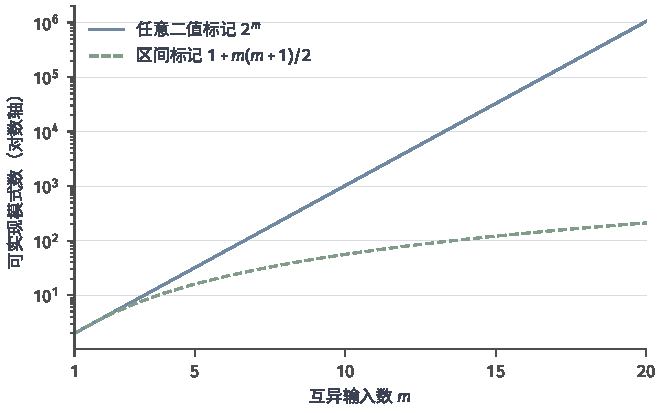
\includegraphics[width=107mm]{figures/06-foundations/02-learning-theory/matplotlib/combinatorics-growth-patterns/figure.pdf}
  \caption{有限输入上的二值模式数（精确计数教学图）。蓝实线为不受限制的\(2^m\)，绿虚线为实数轴区间分类器的\(1+m(m+1)/2\)。纵轴使用对数刻度，绿线是该具体类的精确计数；它也恰等于至多两个正类点的集合族计数，但两类实现的模式可以不同。}
  \label{fig:combinatorics-growth-patterns}
  \label{fig:learning-sauer-growth}
\end{figure}

这一区别正是学习所需要的。有限空间的样本量界中，$\log|\mathcal H|$是不随$n$变化的常数；对无限空间，下一节的对称化之后起同样作用的是$\log\Pi_{\mathcal H}(2n)$。VC维有限时它不超过$d\log(2en/d)$，只按$\log n$增长，除以$n$后仍趋于零；VC维无限时它等于$2n\log2$，与$n$同阶增长，概率界中的指数衰减被完全抵消。

\section{二分类的可学习性}
\label{sec:binary-learnability-characterization}

前一节只说明了有限输入上能出现多少种预测，还没有说明未来观测上的风险。第~\ref{sec:binary-uniform-convergence}小节已经说明，只要所有假设的风险同时估计准确，ERM在样本上的比较就能转移到总体风险上；对无限假设空间，要控制的仍是这一事件的概率。本节分两步把组合计数接到这一事件上。

有限VC维一侧，借助一份副样本把未来表现转成两份样本中有限位置上的预测模式，再用集中不等式与模式计数控制风险，得到一致收敛，这给出一种成功的办法。无限VC维一侧，把概率质量放在一个大的打散集上，使训练之后仍有许多点的标签无法判断，这说明任何办法都会遇到困难。两侧使用的工具不同，不能由一侧代替另一侧；合起来才是可学习性的刻画。最后给出样本复杂度的最优阶，并分清哪些结论在本章完整证明、哪些引用外部结果。

\subsection{副样本、对称化与一致收敛界}

先看直接套用训练模式计数的缺口。训练输入固定后，$\mathcal H$在这$n$个点上至多有$\Pi_{\mathcal H}(n)$种预测，可是偏差事件$|\hat R_S(h)-R_{\mathcal P}(h)|>\eta$还涉及总体风险。两条规则在训练点上完全相同，经验风险也相同，在未见区域却仍可能不同，总体风险因而不同；阈值0.5与0.6在四封训练邮件上不可区分，在分数0.55的邮件上就给出相反的判断。所以总体风险事件不能只靠这份训练输入上的模式来判断，需要另找一个只涉及有限位置、又能反映未来表现的量。

对称化的想法是：再引入一份同样大小的样本，用两份样本经验风险的差异来控制原样本经验风险与总体风险的差异。具体地，在证明中另外抽取一份与$S=(z_1,\ldots,z_n)$独立且同分布的样本$S'=(z_1',\ldots,z_n')$。这份\term{副样本}（ghost sample）只是分析工具，学习算法并不使用它。

副样本能起这个作用，是因为它没有参与选择假设。若原样本上存在偏差超过$\eta$的候选，先固定其中一个由原样本确定的见证$h$；它只是证明中用来标记坏事件的对象，不必是实际算法的输出。这时副样本与$h$独立，$\hat R_{S'}(h)$是$n$个独立损失的平均，期望恰为$R_{\mathcal P}(h)$，由集中性，样本够大时它以至少$1/2$的概率与$R_{\mathcal P}(h)$相差不到$\eta/2$。若$h$在原样本上的经验风险偏离总体风险超过$\eta$，而在副样本上偏离不到$\eta/2$，两份样本上的经验风险就相差超过$\eta/2$。所以“某个假设在原样本上偏差很大”的概率，至多是“某个假设在两份样本上的经验风险相差很大”的概率的2倍。这一步只需副样本把原样本选出的那一个见证估计准确，不要求它同时估计准确所有假设；它用一个概率比较把未来表现连接到$2n$个有限位置上的损失，并没有把一份副样本直接等同于总体。

把比较搬到两份样本上之后，先固定两份样本合并后的$2n$条观测。此时每个候选在这些位置上的损失都已确定，在这$2n$个输入上预测相同的两个假设，在两份样本上的经验风险也分别相同。但一旦固定了观测，两份样本上的经验风险之差就是一个确定的数，无从谈论它偏大的概率。剩下可以利用的随机性是“哪一条观测落入训练一侧、哪一条落入副样本一侧”。为此，对每一对观测$(z_i,z_i')$独立地以各一半的概率决定是否交换二者的位置。原样本与副样本独立同分布，交换任何一对都不改变两份样本的联合分布，所以交换后的差值与原来的差值同分布。而对一个固定的候选，交换后两侧平均损失的差只随交换变化，是$n$个独立随机符号乘以有界项之和，正是Hoeffding不等式能处理的形式。最后，差值只由候选在$2n$个输入上的预测模式决定，对至多$\Pi_{\mathcal H}(2n)$种模式取并集，再用Sauer--Shelah引理控制这个数量。

图~\ref{fig:lt5-symmetrization-swap}用四对观测说明这一机制。固定一个假设，它在原样本上的损失为$(1,0,1,0)$，在副样本上为$(1,1,0,0)$，两份经验风险都是0.5，差为零。只交换第3对，原样本一侧的损失变为$(1,0,0,0)$，副样本一侧变为$(1,1,1,0)$，差变为0.5。第1、4对的两条损失相同，交换与否都不影响差值；第2、3对的损失不同，交换时差值的对应项变号。记$\sigma_i\in\{1,-1\}$表示第$i$对保持或交换，差值等于$(\sigma_2-\sigma_3)/4$，在$-0.5$、$0$、$0.5$上的概率为$1/4$、$1/2$、$1/4$。

\begin{figure}[htbp]
  \centering
  % 对称化中原样本与副样本的逐对交换（第5章5.3.1）。教学数值：固定一个假设 h，n=4 对观测。
% 原样本损失 l_i = (1,0,1,0)，副样本损失 l'_i = (1,1,0,0)；差 a_i = l'_i - l_i = (0,1,-1,0)。
% 交换前：R_S = 2/4 = 0.5，R_S' = 2/4 = 0.5，差为 0。只交换第 3 对（sigma_3=-1）后：
% R_{S_sigma} = 1/4 = 0.25，R_{S'_sigma} = 3/4 = 0.75，差为 0.5。
% sigma 独立等概率取 ±1 时，差 = (sigma_2 - sigma_3)/4 取 -0.5、0、0.5，概率 1/4、1/2、1/4（右下柱高按此比例）。
\begingroup
\begin{tikzpicture}[figure picture,x=1mm,y=1mm,
  err/.style={draw=FigureStroke,line width=.6pt,fill=FigureRedFill,minimum size=6mm,inner sep=0pt},
  ok/.style={draw=FigureStroke,line width=.6pt,fill=white,minimum size=6mm,inner sep=0pt},
  swapped/.style={draw=FigureYellow,line width=1.1pt,rounded corners=1mm}]
\newcommand{\lossRows}[4]{% #1 x0, #2 S losses, #3 S' losses, #4 heading
  \node[figure heading] at (#1+12,45) {#4};
  \foreach \v [count=\i] in {#2}{\ifnum\v=1 \node[err] at (#1+7*\i-7,30) {$1$};\else\node[ok] at (#1+7*\i-7,30) {$0$};\fi}
  \foreach \v [count=\i] in {#3}{\ifnum\v=1 \node[err] at (#1+7*\i-7,22) {$1$};\else\node[ok] at (#1+7*\i-7,22) {$0$};\fi}
  \foreach \i in {1,...,4}{\node[figure note] at (#1+7*\i-7,37.5) {$\i$};}}
\node[anchor=east] at (-4,30) {原样本};
\node[anchor=east] at (-4,22) {副样本};
\node[figure note,anchor=east] at (-4,37.5) {第 $i$ 对};
\lossRows{0}{1,0,1,0}{1,1,0,0}{交换前}
\node[anchor=west] at (24.5,30) {$0.50$};
\node[anchor=west] at (24.5,22) {$0.50$};
\draw[figure flow] (36,26)--(48,26);
\node[figure note] at (42,30) {$\sigma_3=-1$};
\node[figure note] at (42,21.5) {其余 $\sigma_i=1$};
\lossRows{55}{1,0,0,0}{1,1,1,0}{只交换第 3 对}
\draw[swapped] (66.6,18.4) rectangle (73.4,33.6);
\node[anchor=west] at (79.3,30) {$0.25$};
\node[anchor=west] at (79.3,22) {$0.75$};
\node[figure note,anchor=west] at (24.5,36.5) {经验风险};
\node[figure note,anchor=west] at (79.3,36.5) {经验风险};
\node[figure note,anchor=east] at (88,14) {副样本减原样本：$0\ \to\ 0.5$};
% distribution of the difference
\node[figure heading,anchor=west] at (-16,7) {$\sigma$ 随机时差值的分布};
\draw[FigureStroke,line width=.6pt] (-14,-14)--(24,-14);
\foreach \x/\h/\lab/\p in {-6/5/{-0.5}/{1/4},5/10/{0}/{1/2},16/5/{0.5}/{1/4}}{
  \fill[FigureBlueFill] (\x-3,-14) rectangle (\x+3,-14+\h);
  \draw[FigureBlue,line width=.75pt] (\x-3,-14) rectangle (\x+3,-14+\h);
  \node[figure note] at (\x,-17.5) {$\lab$};
  \node at (\x,-14+\h+2.6) {$\p$};}
\node[figure note,anchor=west,align=left] at (32,-7) {只有第 2、3 对的两条损失不同，\\差值 $=(\sigma_2-\sigma_3)/4$；\\第 1、4 对交换与否都不影响};
\end{tikzpicture}
\endgroup

  \caption{原样本与副样本的逐对交换。固定一个假设，格中数字是它在各条观测上的零一损失，红底表示出错；右侧数字为该行的经验风险。黄框标出被交换的第3对。下方是四个随机符号独立等概率取值时，副样本与原样本经验风险之差的分布。}
  \label{fig:lt5-symmetrization-swap}
\end{figure}

交换的作用由此可见：两份样本中的$2n$条观测固定后，差值的随机性完全来自随机符号，而它的大小只取决于各对损失之差。两条损失相同的对不贡献随机性，损失不同的对各贡献一个$\pm1/n$。对每种预测模式施加Hoeffding不等式，再对至多$\Pi_{\mathcal H}(2n)$种模式应用并集界，就控制了“存在某个假设在两份样本上差距很大”的概率。引入副样本与随机交换的做法合称\term{对称化}（symmetrization）：它把与未知总体风险的比较，转化为有限种预测模式加上随机符号的问题。下面的定理按副样本、随机交换和预测计数三步写出这一论证。

\begin{theorem}[VC一致收敛界]
\label{thm:vc-uniform-convergence}
设$(X,\mathcal X)$为可测空间，$Y=\{0,1\}$取离散$\sigma$代数，
$\mathcal H\subseteq Y^X$是由可测分类器组成的非空集合，零一损失函数类
\[
 \mathcal F_{\mathcal H}
 =\{(x,y)\mapsto\mathbb I\{h(x)\neq y\}:h\in\mathcal H\}
\]
中的每个函数均可测，并存在可数子类$\mathcal F_0\subseteq\mathcal F_{\mathcal H}$，
使$\mathcal F_{\mathcal H}$中的每个函数都是$\mathcal F_0$中某个函数序列的逐点极限。
设$\mathcal P$是$X\times Y$上的任意联合分布，$n\geq1$，
$S=((x_i,y_i))_{i=1}^n\sim\mathcal P^n$，$R_{\mathcal P}$、$\hat R_S$为零一损失下的总体与经验风险，$\Pi_{\mathcal H}$为式~\eqref{eq:growth-function}定义的生长函数。
令$d=\operatorname{VC}(\mathcal H)$。对任意$\eta>0$，只要$n\eta^2\geq2$，就有
\begin{equation}
 \mathbb P_{S\sim\mathcal P^n}\left\{
   \sup_{h\in\mathcal H}|R_{\mathcal P}(h)-\hat R_S(h)|>\eta
 \right\}
 \leq4\Pi_{\mathcal H}(2n)e^{-n\eta^2/8}.
 \label{eq:vc-symmetrization-probability}
\end{equation}
因而对任意$\delta\in(0,1)$，当$1\leq d\leq2n$时，以至少$1-\delta$的概率，
\begin{equation}
 \sup_{h\in\mathcal H}|R_{\mathcal P}(h)-\hat R_S(h)|
 \leq
 \sqrt{\frac8n\left[
   d\log\frac{2en}{d}+\log\frac4\delta
 \right]}.
 \label{eq:vc-uniform-bound}
\end{equation}
若右侧大于1，则可用零一损失给出的平凡上界1替代。
\end{theorem}

\begin{proof}
先说明可测性。由逐点逼近，经验平均随之收敛；损失取值于$[0,1]$，由有界收敛定理，总体风险也随之收敛。于是若某个$h\in\mathcal H$满足$|R_{\mathcal P}(h)-\hat R_S(h)|>\eta$，则$\mathcal F_0$中逼近它的函数从某项起也满足同一严格不等式。因此下面出现的各个上确界都可以只在可数子类上计算，相应事件可测；在可数子类的固定枚举中取第一个满足条件的成员，便得到一个随样本可测变化的选择。这正是第~\ref{sec:measurability-convention}节约定的用法。

第一步用副样本代替总体风险。记$A=\{\sup_h|R_{\mathcal P}(h)-\hat R_S(h)|>\eta\}$。在$A$上按上述方式选出$h_S$，使$|R_{\mathcal P}(h_S)-\hat R_S(h_S)|>\eta$。引入与$S$独立的副样本$S'\sim\mathcal P^n$。条件于$S$，$h_S$已经固定，$\hat R_{S'}(h_S)$是$n$个独立Bernoulli损失的平均，均值为$R_{\mathcal P}(h_S)$，方差至多$1/(4n)$。由Chebyshev不等式（可参考\BookChapterRef{chap:sampling-errors}{卷1《数学准备：基础数学》的“抽样分布与估计误差”章}），
\[
 \mathbb P_{S'}\left(
   |\hat R_{S'}(h_S)-R_{\mathcal P}(h_S)|\geq\frac{\eta}{2}
   \,\middle|\,S
 \right)
 \leq\frac{1/(4n)}{\eta^2/4}=\frac{1}{n\eta^2}\leq\frac12,
\]
最后一步用到条件$n\eta^2\geq2$。在$A$上，若副样本偏差小于$\eta/2$，三角不等式给出$|\hat R_{S'}(h_S)-\hat R_S(h_S)|>\eta-\eta/2=\eta/2$。对$S$取平均，
\[
 \mathbb P\left\{\sup_h|\hat R_{S'}(h)-\hat R_S(h)|>\frac\eta2\right\}
 \geq\mathbb E_S\left[\mathbb I_A\cdot\frac12\right]
 =\frac12\mathbb P(A).
\]
即$\mathbb P(A)$不超过双样本差事件概率的2倍。

第二步引入随机交换。对$\sigma\in\{1,-1\}^n$，令$S_\sigma,S_\sigma'$为把$\sigma_i=-1$的各对$(z_i,z_i')$互换位置后得到的两份样本。$2n$条观测独立同分布，互换任意几对不改变$(S,S')$的联合分布，所以对每个固定的$\sigma$，双样本差事件的概率不变；再让$\sigma_1,\ldots,\sigma_n$独立且各以$1/2$的概率取$\pm1$，并与$(S,S')$独立，便有
\[
 \mathbb P\left\{\sup_h|\hat R_{S'}(h)-\hat R_S(h)|>\frac\eta2\right\}
 =\mathbb E_{S,S'}\,\mathbb P_\sigma\left\{\sup_h|\hat R_{S_\sigma'}(h)-\hat R_{S_\sigma}(h)|>\frac\eta2\right\}.
\]
固定$S,S'$与$h$，记$a_i(h)=\ell_{01}(h(x_i'),y_i')-\ell_{01}(h(x_i),y_i)\in\{-1,0,1\}$，则
\[
 \hat R_{S_\sigma'}(h)-\hat R_{S_\sigma}(h)
 =\frac1n\sum_{i=1}^n\sigma_i a_i(h).
\]
各项$\sigma_ia_i(h)/n$独立、均值为零，取值区间长度至多$2/n$，宽度平方和至多$4/n$。Hoeffding不等式分别用于右尾与左尾，得到$\mathbb P_\sigma\{|\cdot|>\eta/2\}\leq2\exp\{-2(\eta/2)^2/(4/n)\}=2e^{-n\eta^2/8}$；若全部$a_i(h)=0$，差恒为零，这个概率为零，上界仍成立。

第三步对预测模式计数。固定$S,S'$后，标签已定，差值向量$\bm a(h)=(a_1(h),\ldots,a_n(h))$只由$h$在$x_1,\ldots,x_n,x_1',\ldots,x_n'$这$2n$个输入上的预测向量决定，所以随$h$遍历$\mathcal H$，它至多取$\Pi_{\mathcal H}(2n)$个不同的值。上确界因而只是对这些有限个向量取最大，并集界给出
\[
 \mathbb P_\sigma\left\{
   \sup_h|\hat R_{S_\sigma'}(h)-\hat R_{S_\sigma}(h)|>\frac\eta2
 \right\}
 \leq2\Pi_{\mathcal H}(2n)e^{-n\eta^2/8}.
\]
这个界对每一对$S,S'$都成立，对它们取平均后不变；乘上第一步的因子2，即得式~\eqref{eq:vc-symmetrization-probability}。

最后，当$1\leq d\leq2n$时，Sauer--Shelah引理给出$\Pi_{\mathcal H}(2n)\leq(2en/d)^d$。令$\eta$等于式~\eqref{eq:vc-uniform-bound}右端，则$n\eta^2/8=d\log(2en/d)+\log(4/\delta)$，式~\eqref{eq:vc-symmetrization-probability}的右端至多为$4(2en/d)^de^{-n\eta^2/8}=\delta$。条件$n\eta^2\geq2$也自动满足：$2en/d\geq e$使$d\log(2en/d)\geq0$，故$n\eta^2\geq8\log4>2$。
\end{proof}

固定有限的$d$和$\delta$，$n\to\infty$时式~\eqref{eq:vc-uniform-bound}的右端趋于零。所以对任意偏差容限$\eta$，都存在一个只依赖$d,\eta,\delta$的样本量，使所有假设的偏差以至少$1-\delta$的概率同时不超过$\eta$，这正是定义~\ref{def:learning-uniform-convergence}的一致收敛。与有限空间的式~\eqref{eq:finite-uniform-bound}对照，$\log|\mathcal H|$的位置换成了$d\log(2en/d)$。

这个界的常数并不紧。以全部实数阈值为例，$d=1$、$\delta=0.05$、$n=10000$时，式~\eqref{eq:vc-uniform-bound}的右端为$\sqrt{8(\log(2e\cdot10^4)+\log80)/10^4}\approx0.11$；而只含四个阈值的有限空间，式~\eqref{eq:finite-uniform-bound}在同样的$n,\delta$下给出约0.016。差距一部分来自模式数随$n$增长（根号内的对数项约大3倍），更多来自对称化的损耗：副样本只以$1/2$的概率把偏差估计准确，比较两份样本时容限又减半，交换后每项的取值区间加倍，这些反映在指数中的$1/8$上，与有限情形的$2$相比差了16倍。反过来看，要使右端降到$0.1$，$d=1$时需要$n=12401$，$d=10$时需要$n=89880$。这个界的作用在于证明一致收敛成立、给出$d$与$n$的依赖关系，而不是给出实用的样本量估计。

\subsection{二分类学习基本定理}

把一致收敛界与前面的结果连起来，就得到VC维与可学习性的等价关系。在第~\ref{sec:measurability-convention}节的可测性约定下，正向的链是：VC维有限推出一致收敛；一致收敛经定理~\ref{thm:approximate-erm-risk}的比较推出ERM的不可知PAC保证；不可知PAC覆盖可实现分布，因而推出可实现PAC。这条链在同一个成功事件上同时控制了所有候选，所以对任意满足要求的经验最优选解都成立，不依赖ERM在并列最优者之间怎样挑选。

反向需要另一种论证：若VC维无限，必须说明任何算法都做不到统一的可实现PAC。这是一个信息下界，机制在第~\ref{sec:no-free-lunch}节已经出现，这里在VC维无限的条件下把它重述一遍。对样本量$n$，VC维无限保证存在一个被打散的$2n$点集合$C$。让输入在$C$上均匀出现，每个点的概率为$1/(2n)$，再把$C$上每个点的目标标签独立地随机指定为0或1，各以$1/2$的概率。由于$C$被打散，每一种指定都由$\mathcal H$中某个分类器实现，所以无论随机指定的结果如何，得到的都是一个对$\mathcal H$可实现、标签没有噪声的分布。

训练样本含$n$条观测，至多见到$n$个不同输入，因此$C$中至少有一半的概率质量落在未见点上。在这些点上，目标标签是独立的公平硬币，和训练中看到的标签没有任何联系；无论学习器在某个未见点上回答0还是1，答错的条件概率都是$1/2$。只累加未见点上的错误，对随机目标平均的风险至少为$(1/2)\times(1/2)=1/4$。图~\ref{fig:lt5-unseen-labels-shattered}对比了$n=3$时的两种情形：被打散的六点上，训练见到三个点后另外三个点仍可任意二选一；阈值类中，同样的已见标签就推出了其中两个点的标签，只剩一个点未定。

\begin{figure}[htbp]
  \centering
  % 训练后仍未定的标签：被打散的六点集与阈值类对比（第5章5.3.2）。教学设定：n=3，|C|=2n=6，
% 输入 x_1<...<x_6 各有概率 1/6。训练样本见到 x_1、x_3、x_5，标签依次为 0、0、1（黄底标出）。
% (a) 类打散 C：未见点 x_2、x_4、x_6 的 8 种补全都可实现，三点全部未定，未定概率质量 3/6=1/2；
%     目标标签取独立公平硬币时，任何输出在每个未见点上的条件错误概率都是 1/2，平均风险至少 1/2*1/2=1/4。
% (b) 右侧判正的阈值 h_t(x)=I{x>=t}：x_3 为 0 推出 x_2 为 0，x_5 为 1 推出 x_6 为 1（浅色），只剩 x_4 未定，质量 1/6。
% 屏幕坐标：点 x_i 位于横坐标 22+11i（毫米）。
\begingroup
\begin{tikzpicture}[figure picture,x=1mm,y=1mm,
  one/.style={circle,fill=FigureBlue,draw=FigureBlue,inner sep=0pt,minimum size=2.8mm},
  zero/.style={circle,fill=white,draw=FigureRed,line width=.75pt,inner sep=0pt,minimum size=2.8mm},
  fone/.style={circle,fill=FigureBlue!40!white,draw=FigureBlue,dashed,line width=.6pt,inner sep=0pt,minimum size=2.8mm},
  fzero/.style={circle,fill=white,draw=FigureRed,dashed,line width=.6pt,inner sep=0pt,minimum size=2.8mm},
  free/.style={circle,fill=white,draw=FigureMuted,dashed,line width=.6pt,inner sep=0pt,minimum size=3.6mm,font=\figurefont\scriptsize\bfseries,text=FigureMuted},
  seen/.style={fill=FigureYellowFill,draw=FigureYellow,line width=.6pt,rounded corners=1mm}]
\node[figure heading,anchor=west] at (0,44) {假设空间};
\node[figure heading] at (61.5,44) {六个等概率输入（$n=3$）};
\node[figure heading] at (100,44) {未定质量};
\foreach \i in {1,...,6}{\node[figure note] at (22+11*\i,39) {$x_{\i}$};}
% 两行共同的已见位置
\foreach \i in {1,3,5}{\draw[seen] (22+11*\i-3.6,31.4) rectangle (22+11*\i+3.6,35.6);
                       \draw[seen] (22+11*\i-3.6,17.4) rectangle (22+11*\i+3.6,21.6);}
% (a) 被打散的集合
\node[anchor=west] at (0,33.5) {(a) 打散这六点};
\draw[FigureStroke] (30,33.5)--(93,33.5);
\node[zero] at (33,33.5) {}; \node[zero] at (55,33.5) {}; \node[one] at (77,33.5) {};
\node[free] at (44,33.5) {?}; \node[free] at (66,33.5) {?}; \node[free] at (88,33.5) {?};
\node at (100,33.5) {$3/6$};
% (b) 阈值
\node[anchor=west] at (0,19.5) {(b) 阈值类};
\draw[FigureStroke] (30,19.5)--(93,19.5);
\node[zero] at (33,19.5) {}; \node[zero] at (55,19.5) {}; \node[one] at (77,19.5) {};
\node[fzero] at (44,19.5) {}; \node[free] at (66,19.5) {?}; \node[fone] at (88,19.5) {};
\node at (100,19.5) {$1/6$};
\draw[FigureMuted,-{Stealth[length=1.6mm]},line width=.5pt] (52.5,16.3) to[bend left=35] (46.5,16.3);
\draw[FigureMuted,-{Stealth[length=1.6mm]},line width=.5pt] (79.5,16.3) to[bend right=35] (85.5,16.3);
% 图例
\node[figure note,anchor=west,align=left] at (0,6) {黄底：训练中出现的输入\quad 实心蓝：标签1\quad 空心红：标签0\\
虚线浅色：由已见标签推出\quad 虚线问号：仍可任意二选一};
\end{tikzpicture}
\endgroup

  \caption{训练后仍未定的标签（$n=3$，六个输入各有概率$1/6$）。训练见到$x_1,x_3,x_5$，标签依次为0、0、1。(a) 若假设空间打散这六点，未见的$x_2,x_4,x_6$上全部8种补全都可实现，未定的概率质量为$1/2$；目标标签取独立公平硬币时，任何输出的平均风险至少为$1/4$。(b) 对右侧判正的阈值，$x_3$为0推出$x_2$为0，$x_5$为1推出$x_6$为1，只剩$x_4$未定，质量为$1/6$，并随样本增多而缩小。}
  \label{fig:lt5-unseen-labels-shattered}
\end{figure}

平均风险的下界还不是PAC意义下的失败，需要恢复第~\ref{sec:no-free-lunch}节下界证明的两步。第一步从目标平均推出一个固定的困难目标：标签指定只有有限多种，若每一种下学习器的期望风险都小于$1/4$，它们的平均也会小于$1/4$，所以必有一种固定的指定$g^\star$，使学习器在相应分布下的期望风险至少为$1/4$。此后训练样本都从这一个固定分布抽取，随机目标不再出现。第二步从期望风险推出常数失败概率：风险$Q$取值于$[0,1]$，记$p=\mathbb P(Q\geq1/8)$，则$1/4\leq\mathbb EQ\leq(1-p)/8+p$，解得$p\geq1/7$。这一论证对任意学习算法成立，包括输出$\mathcal H$以外分类器的算法；它排除的是分布无关的可实现PAC本身，而不只是说明某个ERM会失败。

\begin{theorem}[二分类学习基本定理]
\label{thm:binary-fundamental-theorem}
设$(X,\mathcal X)$为可测空间，$Y=\{0,1\}$取离散$\sigma$代数，
$\mathcal H\subseteq Y^X$是由可测分类器组成的非空假设空间，并采用零一损失。
假定损失类
\[
 \mathcal F_{\mathcal H}
 =\{(x,y)\mapsto\mathbb I\{h(x)\neq y\}:h\in\mathcal H\}
\]
中的每个函数均可测，且存在可数子类$\mathcal F_0\subseteq\mathcal F_{\mathcal H}$，
使$\mathcal F_{\mathcal H}$中的每个函数都是$\mathcal F_0$中某个函数序列的逐点极限。
所有分布均指$X\times Y$上的联合分布，训练样本均为$S\sim\mathcal P^n$；
学习算法是可测映射并输出$\mathcal H$中的分类器，成功概率同时计入样本抽取和算法的
内部随机性。在这一分布无关设定中，下列命题等价：
\begin{enumerate}
 \item $\mathcal H$是不可知PAC可学习的；
 \item $\mathcal H$是可实现PAC可学习的；
 \item $\mathcal H$满足一致收敛；
 \item $\operatorname{VC}(\mathcal H)<\infty$。
\end{enumerate}
\end{theorem}

\begin{proof}
由4推3。VC维为正且有限时，定理~\ref{thm:vc-uniform-convergence}直接给出一致收敛。VC维为0时，没有单点被打散，每个输入处所有假设的预测相同，$\mathcal H$在$X$上实际只有一个预测规则，所有假设的经验风险与总体风险分别相同；对这一个规则用式~\eqref{eq:hoeffding-fixed-hypothesis}，即得一致收敛。

由3推1。零一经验风险只取$0,1/n,\ldots,1$这有限个值，所以类内经验风险的最小值总能取到；按可数子类的固定枚举取第一个达到最小值的成员，得到可测的ERM。固定一致收敛的成功事件，在其上所有假设的偏差至多$\eta$，定理~\ref{thm:approximate-erm-risk}以$\alpha=0$给出超额风险至多$2\eta$。取$\eta=\varepsilon/2$，样本量取$m_{\mathcal H}^{\mathrm{UC}}(\varepsilon/2,\delta)$，即得不可知PAC。这一论证只用到“输出的经验风险最小”，所以对任意可测的ERM选法都成立。

由1推2。可实现分布的类内最低风险为零，不可知保证在这些分布上就是可实现保证。

由2推4，取逆否。设VC维无限，并假设某算法$A$与样本量函数$m$满足可实现PAC。取$\varepsilon=1/16$、$\delta=1/8$，令$n=\max\{m(1/16,1/8),1\}$，按定义它也满足PAC保证。VC维无限，存在被打散的$2n$点集合，定理~\ref{thm:no-free-lunch-classification}按上面的两步对$A$和这个$n$给出一个可实现分布，使$A$以至少$1/7>1/8$的概率输出风险至少$1/8>1/16$的分类器，与假设矛盾。

四个方向合起来构成一个环，命题两两等价。
\end{proof}

这个定理把第~\ref{chap:statistical-learning-framework}章抽象定义的PAC可学习性归结为一个组合条件：要判断一个二分类假设空间能否在所有分布上被统一地学习，只需判断它的VC维是否有限。阈值、区间与平面半空间的VC维分别为1、2、3，因而都可学习；第~\ref{sec:binary-shattering-vc}小节由二进制位定义的类VC维无穷，任何算法都学不会。

定理的适用范围也要读清楚。必要性证明中的随机目标只是说明困难来源存在的工具：每一种固定的标签指定都给出一个无噪声的可实现分布，随机性只用来在这些分布之间取平均，并不表示可实现学习问题本身加入了随机标签噪声。定理固定了二元标签、零一损失、恰当输出和全部联合分布（或全部可实现分布）这一分布族；必要性一侧借用的没有免费的午餐定理对非恰当输出同样成立，所以VC维无限时允许输出$\mathcal H$以外的分类器也无济于事。标签多于两个、损失换成实值或只允许部分分布时，这些等价关系要重新核对：第~\ref{chap:multiclass-learnability}章会看到，多分类中一致收敛与可学习性可以分离。定理也只回答能否学习；要知道最少需要多少样本，还需要相互匹配的上界和下界。

\subsection{风险上界与最优样本复杂度}

基本定理只回答能否学习。要问最少需要多少样本，先分清两类结论各回答什么。算法上界给出一种具体办法，并说明样本达到某个量时它就成功；它只说明这么多样本够用，不说明更少就不行。信息下界说明，样本少于某个量时，任何办法都可能在某个允许的分布上失败；它不提供成功的办法。只有两侧在指定的参数范围内阶数相同，才能称该阶为最优样本复杂度。上一小节的必要性论证就是一种信息下界，但它只说明VC维无限时不可学习，没有给出样本量随$d$、$\varepsilon$、$\delta$变化的阶。

先看本章VC偏差界能给出什么上界。对不可知ERM，要求式~\eqref{eq:vc-uniform-bound}右端不超过$\varepsilon/2$，即
\[
 n\geq\frac{32}{\varepsilon^2}\left[d\log\frac{2en}{d}+\log\frac4\delta\right]
\]
（同时满足$1\leq d\leq2n$）。右端只随$n$对数增长，所以这样的$n$一定存在；反解可知它的阶为$O\bigl((d\log(d/\varepsilon)+\log(1/\delta))/\varepsilon^2\bigr)$。与有限空间的式~\eqref{eq:finite-agnostic-sample}相比，$\log|\mathcal H|$换成了$d\log(d/\varepsilon)$，多出的$\log(1/\varepsilon)$来自生长函数的计数随样本量增长。这个上界只是本章的分析路线给出的充分样本量。下面的定理对照已有文献结果，列出可实现与不可知两种情形中上下界匹配的最优阶。

\begin{theorem}[二分类的最优样本复杂度阶]
\label{thm:binary-optimal-sample-complexity}
存在普适常数$c_0\in(0,1/2)$，使以下结论成立。设$(X,\mathcal X)$为可测空间，
$Y=\{0,1\}$取离散$\sigma$代数，$\mathcal H\subseteq Y^X$是由可测分类器组成的
非空假设空间，$2\leq d=\operatorname{VC}(\mathcal H)<\infty$。假定零一损失类中的
函数均可测，并存在可数损失子类，使每个损失函数都是该子类中某个函数序列的逐点极限。
对所有$\varepsilon,\delta\in(0,c_0]$，令训练样本$S\sim\mathcal P^n$，其中
$\mathcal P$遍历$X\times Y$上的联合分布，成功概率同时计入样本抽取和学习算法的
内部随机性。这里的极小极大次序是：先固定同一学习算法，再看它在全部允许分布上的最坏样本需求，最后在所有算法中取最小者。在允许算法输出任意可测二分类器的分布无关极小极大意义下，可实现PAC学习的
最优样本复杂度阶为
\[
 \Theta\left(\frac{d+\log(1/\delta)}{\varepsilon}\right),
\]
不可知PAC学习的最优样本复杂度阶为
\[
 \Theta\left(\frac{d+\log(1/\delta)}{\varepsilon^2}\right).
\]
这里的$\Theta$上下界常数均为与$\mathcal H,\varepsilon,\delta$无关的普适常数。
\end{theorem}

本章不证明这个定理，只引用文献中的结论\scite{shalevshwartz2014,hanneke2016optimal}。它的条件需要逐项读清：VC维至少为2，$\varepsilon,\delta$不超过某个普适常数，允许非恰当输出，量词次序是先固定算法再取最坏分布。$d=0,1$的情形需另外处理。上界与下界的来源不同。不可知情形的上界可由ERM配合比本章更精细的一致收敛分析达到，下界来自构造困难分布的信息论证。可实现情形中，经典的ERM分析得到的样本量多出一个$\log(1/\varepsilon)$因子；去掉它需要专门设计的非恰当学习器\scite{hanneke2016optimal}，因此并非任意ERM或恰当学习器都能达到上述阶。

把本节的结论按依据分开，便于后文引用时不越界。完整证明的是：有限类的两个样本量界、Sauer--Shelah引理、VC一致收敛界及基本定理的四个蕴含，其中必要性借用第~\ref{sec:no-free-lunch}节已证明的定理。直接推论是：上面由VC界反解出的$O\bigl((d\log(d/\varepsilon)+\log(1/\delta))/\varepsilon^2\bigr)$充分样本量；它对可实现分布同样适用，但对精度的依赖仍是$1/\varepsilon^2$，比可实现的最优阶差一个$1/\varepsilon$因子，因为本章的VC界没有利用“存在零风险假设”。只引用而未证明的是：可实现情形含$\log(1/\varepsilon)$的经典ERM上界，以及定理~\ref{thm:binary-optimal-sample-complexity}中两个$\Theta$阶，包括去掉对数因子的上界和匹配的下界。三类结论都只讲样本，不讲计算：统计上的最优样本量并不意味着存在高效的算法，计算问题是下一节的内容。

\section{二分类学习的计算条件}
\label{sec:computable-binary-learning}

前面的统计界说明“有足够数据时什么输出会可靠”：样本足够多时，ERM选出的假设总体风险低。但$\argmin_{h\in\mathcal H}\hat R_S(h)$只规定了要找什么，没有给出一个会停机的寻找程序；VC维有限也不会自动给出这样的程序。例如，无限多个候选可以逐个枚举，程序却未必能判断当前找到的经验错误率是否已经最小；即使候选只有有限个、可以穷举，枚举也可能耗费指数时间。

第~\ref{sec:computable-pac}节已经建立了这里需要的语言：输入、标签和预测规则的有效表示，在统计保证之上加入训练与预测都停机的可计算PAC（定义~\ref{def:computable-pac-learning}），以及样本量、训练时间、输出长度与预测时间都有多项式上界的高效PAC（定义~\ref{def:efficient-pac-learning}）。本节沿用这些表示与约定，不重复定义，依次讨论三个问题：能否实际返回答案（第~\ref{sec:binary-computable-erm}小节），能否找到“哪种标记实现不了”这样的组合见证（第~\ref{sec:binary-effective-vc}小节），以及怎样利用问题结构免去昂贵的枚举（第~\ref{sec:binary-efficient-structure}小节）。讨论可计算性时取$X=\mathbb N$、$Y=\{0,1\}$，假设由对每个自然数都停机的预测程序表示，学习器输出这样一个程序的编码；讨论效率时的例子使用有限维布尔输入。

\subsection{可计算ERM的充分条件}
\label{sec:binary-computable-erm}

最直接的路线是：如果已经有一个程序能对每份有限样本求出ERM，再加上有限VC维提供的一致收敛，统计保证就落实为程序。下面的定理把这两个条件分开写出。

\begin{theorem}[可计算ERM给出的学习保证]
\label{thm:computable-erm-pac}
在离散空间$X=\mathbb N$、$Y=\{0,1\}$上采用零一损失。设非空假设空间
$\mathcal H\subseteq Y^X$满足$d=\operatorname{VC}(\mathcal H)<\infty$，并存在
确定性程序$A$，它对每份有限带标签样本$S=((x_i,y_i))_{i=1}^n$都停机，输出
$A(S)\in\mathcal H$的程序编码；该输出程序对每个$x\in\mathbb N$都停机，且
\[
 \hat R_S(A(S))
 =\min_{h\in\mathcal H}\frac1n\sum_{i=1}^n\mathbb I\{h(x_i)\neq y_i\}.
\]
则存在可计算的样本量上界$m(d,\varepsilon,\delta)$，使任意
$\varepsilon,\delta\in(0,1)$、任意$\mathbb N\times Y$上的联合分布$\mathcal P$、
任意$n\geq m(d,\varepsilon,\delta)$及$S\sim\mathcal P^n$均满足
\[
 \mathbb P_{S\sim\mathcal P^n}\left\{
 R_{\mathcal P}(A(S))
 \leq\inf_{h\in\mathcal H}R_{\mathcal P}(h)+\varepsilon
 \right\}\geq1-\delta,
\]
其中$R_{\mathcal P}$为零一损失期望风险。因此，$\mathcal H$恰当地不可知CPAC可学习，
且具有可计算的样本量上界；概率仅来自独立同分布样本。
\end{theorem}

\begin{proof}
统计部分：$X=\mathbb N$可数，取离散$\sigma$代数时任何分类器都可测，可数逼近条件也成立：对每个$k$及$\mathcal H$在$\{0,\ldots,k\}$上的每种模式各取一个代表，得到可数子类；任一$h\in\mathcal H$都是在$\{0,\ldots,k\}$上与它一致的代表当$k\to\infty$时的逐点极限，损失函数随之逐点收敛。若$d\geq1$，定理~\ref{thm:vc-uniform-convergence}给出：只要$n$满足
\[
 \frac{8}{n}\left[d\log\frac{2en}{d}+\log\frac4\delta\right]\leq\frac{\varepsilon^2}{4}
 \quad\text{且}\quad n\geq d/2,
\]
全部偏差不超过$\varepsilon/2$的概率至少为$1-\delta$；$d=0$时用式~\eqref{eq:hoeffding-fixed-hypothesis}得到同样的结论。在这个事件上，$A(S)$的经验风险等于类内最小值，定理~\ref{thm:approximate-erm-risk}以$\eta=\varepsilon/2$、$\alpha=0$给出所需的风险保证。

计算部分：上式左端可用有理运算与对数的任意精度近似逐个$n$地检验，从$n=1$起递增，第一个满足条件的$n$就是$m(d,\varepsilon,\delta)$；左端随$n$增大最终趋于零，所以这一搜索停机。训练停机与输出程序在每个输入上停机，分别由题设对$A$和对其输出的要求保证。
\end{proof}

按第~\ref{sec:computable-pac}节的说法，这个定理给出的是\term{可计算PAC可学习的}（computably PAC learnable）空间的一个充分条件，而且是恰当的、带可计算样本上界的版本。两项停机要求各有出处：训练停机来自假定的ERM程序，预测停机来自它输出的是总可计算程序。统计条件只提供“样本够多时ERM的输出风险低”，不提供其中任何一项。

定理中的“可计算样本量上界”要与一个更强的要求区分。对一个固定的假设空间，只要把它的某个VC维上界作为常数写进程序，就能计算样本量；而根据任意假设空间的程序描述自动算出它的VC维，是强得多的要求，定理的证明并没有提供这种能力。

定理的另一个条件，即存在停机的ERM程序，也不能由“候选可以逐个列出”代替。设$\mathcal H$由一列总可计算程序$h_1,h_2,\ldots$给出。在与某个$h_j$一致的样本上，依次检查$h_1,h_2,\ldots$并停在第一个训练错误为零的候选，这个搜索一定停机，因为零是经验风险能取到的最小值，找到即可确认。有噪声时情况不同：当前找到的最好候选可能仍有错误，例如训练错误为$2/n$，尚未检查的候选中可能有错误为$1/n$的，程序在有限步内无法确认已经找到最小值。数学上存在经验最优的候选，不等于有程序能把它找出来。

\subsection{有效VC维与计算刻画}
\label{sec:binary-effective-vc}

普通VC维为$d$只保证：在任意$d+1$个不同输入上，至少有一种标记是假设空间实现不了的。这是一个存在性陈述：知道某个输入集上有一种标记不能实现，并不等于已有程序能把它找出来。程序若要利用这一事实，例如用它来排除某些候选或构造学习器，就必须在有限时间内把这样一种标记实际找出来。\term{有效VC维}（effective VC dimension）在这一存在性之外再加一个要求：存在一个统一的程序，对任意$d+1$个输入都能返回一种实现不了的标记，作为见证。

\begin{definition}[有效VC维]
\label{def:effective-vc-dimension}
对$\mathcal H\subseteq\{0,1\}^{\mathbb N}$，若存在总可计算映射
$W$，使任意$d+1$个互异输入$x_1,\ldots,x_{d+1}$都满足
\[
 W(x_1,\ldots,x_{d+1})\in\{0,1\}^{d+1}
 \setminus\{(h(x_1),\ldots,h(x_{d+1})):h\in\mathcal H\},
\]
则称$d$为有效VC维的一个上界。所有这样的非负整数$d$中的最小值记为
$\operatorname{eVC}(\mathcal H)$；若不存在，则记为$\infty$。
\end{definition}

$W$只需返回一种实现不了的标记，不必列出全部。以自然数上的递增阈值$h_t(x)=\mathbb I\{x\geq t\}$为例：对任意两个不同的输入，“较小者为1、较大者为0”一定实现不了，因为$h_t$在较小者处为1意味着$t$不超过较小者，于是较大者处也为1。见证程序先比较两个输入的大小，再返回“较小点为1、较大点为0”，一步比较之后就停机，所以有效VC维至多为1；又因为单个输入既可取0也可取1，普通VC维和有效VC维都等于1。图~\ref{fig:lt5-effective-vc-witness}上半部分画出输入$(7,3)$时的返回过程：$W(7,3)=(0,1)$，即把较小的3标为1、较大的7标为0。定义只要求见证程序对每组输入都停机，尚未要求它在多项式时间内完成；资源问题留给第~\ref{sec:binary-efficient-structure}小节。

\begin{figure}[htbp]
  \centering
  % 自然数阈值 h_t(x)=I{x>=t} 的有效 VC 见证（第5章5.4.2）。示例输入 (7,3)，d=1。
% 上行：直接见证程序 W 比较两数大小，返回“较小者为 1、较大者为 0”，即 W(7,3)=(0,1)。
% 下行：由可计算 ERM 得到见证：枚举 (3,7) 上的 2^2=4 种标记，各运行一次 ERM 并计算最小训练错误；
%   (0,0)、(0,1)、(1,1) 的最小错误为 0，(1,0) 的最小错误为 1/2>0，返回第一个错误为正的标记。
\begingroup
\begin{tikzpicture}[figure picture,x=1mm,y=1mm,
  witness step/.style={figure node,minimum height=9mm,draw=FigureBlue,fill=FigureBlueFill},
  witness out/.style={figure node,minimum height=9mm,draw=FigureYellow,fill=FigureYellowFill}]
\node[figure heading,anchor=west] at (0,46) {直接见证：比较大小};
\node[figure node,minimum height=9mm] (in) at (12,36) {输入 $(7,3)$};
\node[witness step,align=center] (cmp) at (47,36) {比较：$3<7$};
\node[witness out,align=center] (w) at (88,36) {$W(7,3)=(0,1)$\\较小的 $3$ 标 1};
\draw[figure flow] (in)--(cmp);\draw[figure flow] (cmp)--(w);
\node[figure note] at (47,28) {若 $h_t(3)=1$，则 $t\leq3<7$，必有 $h_t(7)=1$};
\node[figure heading,anchor=west] at (0,19) {由 ERM 得到见证：逐个检查 $(3,7)$ 上的 4 种标记};
\foreach \lab/\r/\ok [count=\k] in {{(0,0)}/0/1,{(0,1)}/0/1,{(1,0)}/{1/2}/0,{(1,1)}/0/1}{
  \pgfmathsetmacro{\x}{12+22*(\k-1)}
  \ifnum\ok=1
    \node[figure node,minimum width=18mm,minimum height=11mm,align=center] at (\x,6) {$\lab$\\最小错误 $\r$};
  \else
    \node[figure node,minimum width=18mm,minimum height=11mm,align=center,draw=FigureRed,fill=FigureRedFill,line width=1pt] (bad) at (\x,6) {$\lab$\\最小错误 $\r$};
  \fi}
\node[figure note] (ret) at (56,-7) {返回第一个最小错误为正的标记};
\draw[figure flow] (ret.north)--(bad.south);
\end{tikzpicture}
\endgroup

  \caption{自然数阈值的有效VC见证。上：直接见证程序比较两个输入的大小，返回“较小者为1、较大者为0”。下：若有停机的ERM程序，也可以逐个检查$(3,7)$上的四种标记，对每种标记运行ERM并计算最小训练错误；只有$(1,0)$的最小错误为正，它就是返回的见证。}
  \label{fig:lt5-effective-vc-witness}
\end{figure}

图的下半部分显示另一种取得见证的方式：若已有停机的ERM程序，就把每种标记当作一份训练样本交给它，计算输出的训练错误。一种标记可实现，当且仅当类内有假设判对它，即最小训练错误为零；所以第一个最小错误为正的标记就是见证。下面的定理把这两个方向写成两种维数的比较。

\begin{theorem}[普通VC维与有效VC维的比较]
\label{thm:effective-vc-comparison}
设$\mathcal H\subseteq\{0,1\}^{\mathbb N}$非空，$\operatorname{eVC}(\mathcal H)$按定义~\ref{def:effective-vc-dimension}确定。则
$\operatorname{VC}(\mathcal H)\leq\operatorname{eVC}(\mathcal H)$。
若普通VC维有限，且存在一个对每份有限带标签样本都停机的程序，输出$\mathcal H$中
对每个自然数输入都停机、且零一经验风险最小的假设，则两者相等。
\end{theorem}

\begin{proof}
设$d$是有效VC维的一个上界。有效见证对任意$d+1$个互异输入返回一种不可实现的标记，所以没有$d+1$点集合被打散，普通VC维至多为$d$。对所有这样的$d$取最小，得到第一项结论；有效VC维为无穷时结论平凡。

设普通VC维$d<\infty$，并有题设的ERM程序。给定$d+1$个互异输入，按固定次序枚举$2^{d+1}$种标记；对每种标记把它当作样本运行ERM，再在这$d+1$个输入上运行输出的程序，计算训练错误。各步骤都停机。由于$d+1$个点不能被打散，至少一种标记不可实现；对这种标记，类内每个假设至少错一个点，ERM输出的训练错误为正。可实现的标记则有假设全部判对，ERM输出的训练错误为零。所以返回第一个训练错误为正的标记，构成一个总可计算的见证，有效VC维至多为$d$。与第一项结论合并，两者相等。
\end{proof}

上面的定理只在已有ERM程序时把两种维数等同起来；没有这个前提时，二者可以不同。在输入为自然数、输出为总可计算程序的上述模型中，Delle Rose等人证明：非恰当不可知CPAC可学习，当且仅当有效VC维有限\scite{dellerose2023}。本章不重复这一证明。充分性需要另行构造可计算的学习器，普通VC维给出的一致收敛不能代替这一步；引用这一外部刻画，只为说明有效见证承担的作用。

这一刻画允许非恰当输出，不能直接替换成要求输出属于$\mathcal H$的恰当版本。样本量上界也要区分两个层次：对某个给定的可计算学习器，统计定义只要求充分样本量存在，不保证能计算它；但对假设类的存在性而言，上述研究同时证明，非恰当CPAC可学习等价于存在一个具有可计算样本上界的非恰当学习器。这里可以更换学习器，不是说原来那个学习器的样本界突然变得可算。要求恰当输出后，这两种要求则可能分离\scite{dellerose2023}。由$\operatorname{VC}(\mathcal H)\leq\operatorname{eVC}(\mathcal H)$，有效VC维有限推出普通VC维有限，反方向一般还缺少计算条件：确实存在普通VC维有限、却不能由非恰当总可计算学习器学到的假设类，按上述刻画，它们的有效VC维必为无限。对这些类，统计信息已经足够，但没有满足要求的总可计算学习程序；这与下一小节讨论的“程序能停机却太慢”是不同的障碍。

\subsection{利用结构实现高效学习}
\label{sec:binary-efficient-structure}

程序能停机，仍可能慢到无法使用。高效PAC学习（定义~\ref{def:efficient-pac-learning}）进一步要求样本量、训练时间、输出长度和预测时间都是规模参数的多项式。有限假设空间是最容易看清统计成本与计算成本差别的地方：样本量随$\log|\mathcal H|$增长，逐个枚举却随$|\mathcal H|$本身增长。下面用布尔合取说明，怎样利用问题结构避开枚举。

\paragraph{布尔合取的候选与枚举代价}
输入为$\bm x\in\{0,1\}^p$。文字指某个坐标$x_j$或它的否定$\neg x_j$（取值$1-x_j$）；合取由若干文字组成，在所选文字全为1时预测1，否则预测0。例如$p=3$时，$x_1\wedge\neg x_3$把$(1,0,0)$和$(1,1,0)$判为1，其余输入判为0。每个坐标可以选正文字、负文字或不选，所以不含矛盾文字的合取恰有$3^p$个（其中不选任何文字的空合取恒为1），再加上恒为0的假设，组成假设空间$\mathcal C_p$，$|\mathcal C_p|=3^p+1$。

代入有限类的可实现样本量界，取$\varepsilon=0.1$、$\delta=0.05$：$p=3$时$|\mathcal C_3|=28$，充分样本量为$\lceil(\log28+\log20)/0.1\rceil=64$；$p=100$时，因为$\log(3^{100}+1)\approx100\log3$，充分样本量约为1129。样本量只随$p$线性增长，逐个检查却要面对约$5\times10^{47}$个候选。困难在于求解方式，而不在于所需的数据量。

\paragraph{从全部文字开始删除}
在可实现样本上，可以不经枚举直接构造一个一致的合取。思路是从限制最严的合取出发，只在证据迫使时放松。先保留全部$2p$个文字，此时合取同时含$x_j$与$\neg x_j$，恒为0。然后依次扫描每个正例，删去在该正例上取0的文字，因为保留它们会把这个正例错判为0。负例不改动文字。最后输出剩余文字组成的合取；若文字全部被删去，输出恒为1；若样本中没有正例，输出恒为0。

图~\ref{fig:lt5-conjunction-elimination}用$p=3$逐步演示。样本由学习器不知道的目标$x_1\wedge\neg x_3$标注。第一个正例$(1,0,0)$删去在它上面取0的$\neg x_1$、$x_2$、$x_3$，剩下$x_1\wedge\neg x_2\wedge\neg x_3$。第二条是负例$(0,1,0)$，当前合取在它上面为0，判断正确，不改动。第三条是正例$(1,1,0)$，删去$\neg x_2$，剩下$x_1\wedge\neg x_3$。第四条是负例$(1,1,1)$，当前合取因$\neg x_3$为0而判0，正确。四步之后，输出恰好是目标；一般情况下输出不一定等于目标，但一定与样本一致。

\begin{figure*}[htbp]
  \centering
  % 布尔合取的删除式学习（第5章5.4.3）。p=3，目标合取 x1 ∧ ¬x3（学习器不知道）。
% 样本：(1,0,0)->1，(0,1,0)->0，(1,1,0)->1，(1,1,1)->0（均由目标合取标注）。
% 每读到正例，删去在该输入上取 0 的文字；负例不改动文字，只用于核对。
% 编码：蓝底=保留；红底带斜线=本步删除；灰色空格=此前已删除。
% 步1删去 ¬x1、x2、x3；步3删去 ¬x2；最终保留 x1、¬x3。
\begingroup
\begin{tikzpicture}[figure picture,x=1mm,y=1mm,
  keep/.style={draw=FigureBlue,fill=FigureBlueFill,line width=.6pt,minimum width=9mm,minimum height=6mm,inner sep=0pt},
  drop/.style={draw=FigureRed,fill=FigureRedFill,line width=.6pt,minimum width=9mm,minimum height=6mm,inner sep=0pt},
  gone/.style={draw=FigureGrid,fill=white,line width=.6pt,minimum width=9mm,minimum height=6mm,inner sep=0pt,text=FigureGrid}]
\foreach \lit [count=\j] in {x_1,\neg x_1,x_2,\neg x_2,x_3,\neg x_3}{
  \node[figure heading] at (30+10*\j,42) {$\lit$};}
\node[figure heading] at (3,42) {步骤};
\node[figure heading] at (19,42) {输入，标签};
\node[figure heading] at (113,42) {当前合取};
% state codes: k keep, d dropped now, g gone earlier
\foreach \row/\step/\inp/\codes/\conj in {
  0/初始/{全部 $6$ 个文字}/{k,k,k,k,k,k}/{恒为 $0$},
  1/1/{$(1,0,0)$，$1$}/{k,d,d,k,d,k}/{$x_1\wedge\neg x_2\wedge\neg x_3$},
  2/2/{$(0,1,0)$，$0$}/{k,g,g,k,g,k}/{不变；预测 $0$ 正确},
  3/3/{$(1,1,0)$，$1$}/{k,g,g,d,g,k}/{$x_1\wedge\neg x_3$},
  4/4/{$(1,1,1)$，$0$}/{k,g,g,g,g,k}/{不变；预测 $0$ 正确}}{
  \pgfmathsetmacro{\y}{34-8*\row}
  \node at (3,\y) {\step};
  \node at (19,\y) {\inp};
  \foreach \c [count=\j] in \codes {
    \if k\c \node[keep] at (30+10*\j,\y) {};\fi
    \if d\c \node[drop] (dd) at (30+10*\j,\y) {};\draw[FigureRed,line width=.75pt] (dd.south west)--(dd.north east);\fi
    \if g\c \node[gone] at (30+10*\j,\y) {};\fi}
  \node at (113,\y) {\conj};}
\node[figure note,anchor=west] at (0,-6) {蓝：保留；红斜线：本步删除；灰空格：此前已删除。负例只用于核对，不改动文字。};
\end{tikzpicture}
\endgroup

  \caption{布尔合取的删除式学习（$p=3$，目标合取$x_1\wedge\neg x_3$对学习器未知）。每行是一步，六列对应六个文字：蓝色为保留，红色斜线为本步删除，灰色空格为此前已删除。正例删去在其上取0的文字；负例只用于核对当前合取的预测。最右列是每步之后的合取。}
  \label{fig:lt5-conjunction-elimination}
\end{figure*}

\begin{theorem}[布尔合取的高效可实现学习]
\label{thm:efficient-conjunction-learning}
设$p,n\geq1$，$X=\{0,1\}^p$、$Y=\{0,1\}$均取离散$\sigma$代数，
$\mathcal C_p$由$X$上的无矛盾布尔合取（包括空合取给出的恒为1假设）及恒为0假设组成。
对样本$S=((\bm x_i,y_i))_{i=1}^n$，确定性学习算法先保留全部$2p$个正、负文字；
每读到一个正例，
便删除在该输入上取0的文字；若样本没有正例则输出恒为0，否则输出剩余文字的合取，
没有剩余文字时输出恒为1。该算法在$\mathcal C_p$可实现的样本上输出与样本一致的
假设，训练时间为$O(np)$，预测时间为$O(p)$。若$\mathcal P$是$X\times Y$上的
联合分布，存在$h^\star\in\mathcal C_p$满足
$\mathbb P_{(x,y)\sim\mathcal P}\{h^\star(x)\neq y\}=0$，且$S\sim\mathcal P^n$，
则对任意$\varepsilon,\delta\in(0,1)$，只要
\[
 n\geq\frac{\log(3^p+1)+\log(1/\delta)}{\varepsilon},
\]
就以关于$S\sim\mathcal P^n$至少$1-\delta$的概率输出零一损失期望风险不超过
$\varepsilon$的假设。
\end{theorem}

\begin{proof}
先证一致性。设样本由某个$h^\star\in\mathcal C_p$判对。无正例时，恒为0判对全部负例。有正例时$h^\star$不是恒为0，它是一个无矛盾合取，它的每个文字在所有正例上都为1，因此从不被删除，剩余文字包含$h^\star$的全部文字。剩余文字也全在正例上为1，否则早已被删除，故输出判对全部正例。任意负例上，$h^\star$至少有一个文字为0；这个文字仍被保留，输出也为0。由此输出与全样本一致。输出还属于$\mathcal C_p$：读过一个正例后，每个坐标的两个文字中至少有一个在该正例上为0而被删除，剩余文字不含矛盾。

再核算资源。每条观测检查至多$2p$个文字，训练耗时$O(np)$；输出至多含$p$个文字，长度$O(p)$，预测时检查这些文字，耗时$O(p)$。最后，概率$1$下样本由$h^\star$判对，输出与样本一致，把$|\mathcal C_p|=3^p+1$代入定理~\ref{thm:finite-realizable-pac}，即得风险保证。
\end{proof}

这个例子同时给出了样本量界、具体算法和运行时间，三者都是$p$、$1/\varepsilon$与$\log(1/\delta)$的多项式：样本量为$O((p+\log(1/\delta))/\varepsilon)$，训练时间是样本量乘以$O(p)$，输出长度与预测时间为$O(p)$。按定义~\ref{def:efficient-pac-learning}，$\mathcal C_p$这一族是高效可实现PAC可学习的。

算法的正确性依赖可实现性：目标合取中的文字在所有正例上都取1，所以不会被删去。若正例标签有噪声，一个本应为负的输入被标成正例，它会删去目标合取中在其上为0的那个文字，被删的文字再也回不来，一致性的证明就不再成立；输出可能退化为过宽的合取。这时必须回到不可知设定：若某个算法在多项式时间内找到经验风险至多比最小值高$\alpha$的合取，定理~\ref{thm:approximate-erm-risk}给出$2\eta+\alpha$的超额风险界，其中$\eta$来自有限类的一致收敛；能否在多项式时间内做到这一点，是与本例不同的计算问题，本章不讨论。

\section{本章小结}
\label{sec:binary-learning-summary}

回到本章开头的问题：训练记录全部分对，为什么仍可能在新样本上出错？因为样本只能排除错误区域被观察到的规则，而算法是在看过样本之后从许多候选中挑选的，某条坏规则可能碰巧通过全部检验。所以风险控制必须覆盖“依据样本选择假设”这一步，而不能只评价一个事先固定的假设。有限计数与VC计数在这一点上做的是同一件事：先算出单个固定候选在样本上蒙混过关的概率，再为全部候选付出代价。有限空间直接按候选数相加，可实现与不可知两种失败事件分别带来$1/\varepsilon$与$1/\varepsilon^2$的精度代价；无限空间改为数有限输入上的预测模式，Sauer--Shelah引理说明VC维有限时模式数只按多项式增长，副样本与逐对交换再把总体风险换成两份样本上的比较，使模式数真正进入概率界。

在本章的可测性条件下，VC维有限、一致收敛、可实现PAC和不可知PAC四者等价，这就是二分类学习基本定理。充分性说明怎样学会：同时控制全部候选，任何经验最优选解都可靠。必要性说明为什么有时学不会：VC维无限时，概率质量可以放在一个大的打散集上，训练后至少一半质量上的标签仍像公平硬币，任何学习器都会以常数概率失败。两侧的证明路线不同，合起来才是刻画。

这些等价关系首先刻画的是候选空间的统计性质，与计算分别属于三个层次。统计上可学习，由有限的普通VC维回答；程序能否在每份样本上停机并输出总可计算的预测规则，需要可计算ERM或有效VC维这样的见证，后者要求“哪种标记实现不了”能由程序找出；资源是否为多项式，还要核算输出表示与预测代价，布尔合取的删除算法给出了一个三项同时满足的例子。三项结论的依据不同，不能由前一项推出后一项。

下一章把标签从两类扩展到有限或无限多类。允许一个输入被改成多个不同的标签之后，“打散”需要重新定义：是只比较两个固定的候选标签，还是允许每个点上任意替换？二分类中VC维同时控制一致收敛与可学习性，多分类中这两件事将要分开，各自需要不同的维数刻画。

\paragraph{扩展阅读}
Vapnik与Chervonenkis的论文给出了频率一致收敛于概率的组合条件，是本章生长函数与对称化论证的源头\scite{vapnik1971}。Shalev-Shwartz与Ben-David的教材系统给出二分类学习基本定理及其定量形式，可与本章的证明对照阅读\scite{shalevshwartz2014}；Hanneke的论文给出可实现情形去掉对数因子的最优样本复杂度构造\scite{hanneke2016optimal}。Delle Rose等人关于有效VC维的研究可用于对照普通PAC、可计算PAC以及要求可计算样本上界的版本\scite{dellerose2023}。这些区别说明，统计基本定理给出的是可学习的存在性条件，并没有给出全部程序步骤。Rademacher复杂度、样本压缩与提升等更一般的分析工具在第~\ref{chap:convex-learning-and-stability}章展开。
